\documentclass[12pt]{cornell}
\pdfoutput=1

% ------------------------------
% Core packages
% ------------------------------
\usepackage{makeidx}
\makeindex
\usepackage{graphicx}
\usepackage{color}
\usepackage{fancyhdr}
\usepackage{float}
\usepackage{listings}
\usepackage{amsfonts, amssymb, amsmath, bm}
\usepackage{tabularx,colortbl}
\usepackage[chapter]{algorithm}
\usepackage{algorithmic}
\usepackage{tocloft}
\usepackage{enumitem}
\usepackage{longtable}
\usepackage{xspace}
\usepackage{tcolorbox}
\usepackage{txfonts}

% ------------------------------
% Hyperlinks (load late)
% ------------------------------
\usepackage[
  breaklinks=true,
  colorlinks=true,
  citecolor=blue,
  linkcolor=blue,
  urlcolor=blue
]{hyperref}

% ------------------------------
% Fonts and theorem-like environments
% ------------------------------
\newfont{\Bp}{msbm10}
\newfont{\BpBig}{msbm10 scaled\magstep2}
\newfont{\FrBig}{eufm10 scaled\magstep1}

% Avoid \openbox clash between txfonts and amsthm
\let\openbox\relax
\usepackage{amsthm}

% Classic theorem/definition (number per chapter)
\newtheorem{theorem}{Theorem}[chapter]
\newtheorem{definition}{Definition}[chapter]

\theoremstyle{definition}

% ===== Requirements =====
\newtheorem{reqF}{Functional Requirement}[chapter]
\renewcommand{\thereqF}{F-\thechapter.\arabic{reqF}}

\newtheorem{reqQ}{Quality Requirement}[chapter]
\renewcommand{\thereqQ}{Q-\thechapter.\arabic{reqQ}}

\newtheorem{reqC}{Constraint Requirement}[chapter]
\renewcommand{\thereqC}{C-\thechapter.\arabic{reqC}}

\newtheorem{reqI}{Interface Requirement}[chapter]
\renewcommand{\thereqI}{I-\thechapter.\arabic{reqI}}

\newtheorem{reqB}{Business Requirement}[chapter]
\renewcommand{\thereqB}{B-\thechapter.\arabic{reqB}}

% ===== Use Cases =====
\newtheorem{useCase}{Use Case}[chapter]
\renewcommand{\theuseCase}{UC-\thechapter.\arabic{useCase}}

% ===== User Stories =====
\newtheorem{userStory}{User Story}[chapter]
\renewcommand{\theuserStory}{US-\thechapter.\arabic{userStory}}

% hyperref names
\providecommand*{\reqFautorefname}{Functional Requirement}
\providecommand*{\reqQautorefname}{Quality Requirement}
\providecommand*{\reqCautorefname}{Constraint Requirement}
\providecommand*{\reqIautorefname}{Interface Requirement}
\providecommand*{\reqBautorefname}{Business Requirement}
\providecommand*{\useCaseautorefname}{Use Case}
\providecommand*{\userStoryautorefname}{User Story}

\providecommand{\reqid}[1]{\textbf{[#1]}}

% ------------------------------
% Versioning
% ------------------------------
\IfFileExists{rrcversion.tex}{\newcommand{\version}{0.4.13}
\newcommand{\commit}{Manual}
\newcommand{\builddate}{\today}
}{
  \newcommand{\version}{v0.0.0}
  \newcommand{\commit}{unknown}
  \newcommand{\builddate}{\today}
}

% ------------------------------
% Glossary
% ------------------------------
\usepackage[toc,section=chapter,numberedsection=autolabel]{glossaries-extra}
\makenoidxglossaries
% rrcGlossary.tex  (entries only)

% ---------- MoSCoW priorities ----------
\newglossaryentry{must}{
  name={MustHave},
  description={This defines the first highest priority requirement. All of the tasks, requirements, or anything that is marked this way are built in the current version.}
}

\newglossaryentry{should}{
  name={ShouldHave},
  description={This defines the second highest priority requirement. The system should implement all of the tasks, requirements, or anything that is marked this way, but if resources are limited, it can be left out of the current version. Build in next version.}
}

\newglossaryentry{could}{
  name={CouldHave},
  description={This defines the third highest priority requirement. The system could implement all of the tasks, requirements, or anything that is marked this way, but if resources are limited, it can be left out of the current and next version. Build in two versions from now.}
}

\newglossaryentry{would}{
  name={WouldHave},
  description={This defines the lowest priority requirement. The system would like to implement all of the tasks, requirements, or anything that is marked this way, but only if resources are available. It can be left out of all future versions.}
}

% ---------- FindIt project terms ----------
\newglossaryentry{findit}{
  name={FindIt System},
  description={The end-to-end asset tracking solution developed by the team, consisting of the FindIt device, LoRaWAN gateway, and cloud-based data management dashboard.}
}

\newglossaryentry{lora}{
  name={LoRa (Long Range)},
  description={A wireless modulation technique that enables long-range, low-power communication between IoT devices using sub-GHz frequency bands.}
}

\newglossaryentry{LoRaWAN}{
  name={LoRaWAN (Long Range Wide Area Network)},
  description={A protocol built on top of LoRa that defines how end devices communicate with gateways and network servers for secure and scalable data transmission.}
}

\newglossaryentry{Wio Tracker 1110}{
  name={Wio Tracker 1110},
  description={The development board used for prototyping the FindIt device. It integrates Semtech’s LR1110 transceiver, GNSS assistance, and LoRa communication interface.}
}

\newglossaryentry{lr1110}{
  name={LR1110},
  description={A Semtech transceiver that supports LoRa and GNSS assistance, enabling hybrid indoor/outdoor tracking and low-power operation.}
}

\newglossaryentry{TTS}{
  name={The Things Stack (TTS)},
  description={An open-source LoRaWAN network server for device registration, session management, and secure routing of uplink/downlink messages.}
}

\newglossaryentry{Gateways}{
  name={Gateway},
  description={A device that receives LoRaWAN packets from trackers and forwards them to the network server via the internet, bridging local RF to cloud.}
}

\newglossaryentry{SupaBase}{
  name={Supabase},
  description={The backend platform (PostgreSQL + REST/Realtime) used to store and query tracker data and power the FindIt API/dashboard.}
}

\newglossaryentry{battery}{
  name={Battery Life Optimization},
  description={Design focus on minimizing energy usage through duty cycling, GNSS assist, and efficient LoRaWAN classes to target >1 year per device.}
}

\newglossaryentry{Asset Tracking}{
  name={Asset Tracking},
  description={Monitoring the location of objects or people using GNSS (outdoor) and signal-based localization (indoor).}
}

\newglossaryentry{GPS}{
  name={GPS (Global Positioning System)},
  description={Satellite-based navigation providing precise outdoor positioning. Used by the tracker when sky visibility is sufficient.}
}

\newglossaryentry{indoorpos}{
  name={Indoor Positioning},
  description={Location estimation in GPS-denied spaces using RSSI triangulation, Wi-Fi fingerprinting, or Bluetooth beacons.}
}

\newglossaryentry{RSSI}{
  name={RSSI (Received Signal Strength Indicator)},
  description={Measured signal power used for distance/proximity inference and coarse indoor localization.}
}

\newglossaryentry{emergencycomm}{
  name={Emergency Communication},
  description={User-initiated alerts (e.g., panic button or Morse-code sequence) transmitted via LoRaWAN for caregiver notification.}
}

\newglossaryentry{Uplink}{
  name={Device Uplink},
  description={Device transmit data to network server.}
}
\newglossaryentry{Downlink}{
  name={Device Downlink},
  description={Network server transmits data to device.}
}

\newglossaryentry{coverage}{
  name={Gateway Network Coverage},
  description={Geographic area within which gateways can reliably receive tracker signals, determining communication reach and reliability.}
}

\newglossaryentry{purchase}{
  name={One-Time Purchase Model},
  description={Fixed device cost (e.g., \$50) with optional subscription tiers for extended history, private hosting, or premium features.}
}

\newglossaryentry{firmware}{
  name={Firmware},
  description={Embedded software on the tracker controlling sensing, power management, and LoRaWAN communication.}
}

\newglossaryentry{ui}{
  name={User Interface (UI)},
  description={Mobile/web interface for viewing locations, receiving alerts, and managing settings.}
}


% ------------------------------
% Include control
% ------------------------------
\includeonly{
  prologue,
  rrcIntroduction,
  rrcDevelopmentPlan,
  rrcRequirements,
  rrcUserStories,
  rrcUseCases,
  rrcUserInterfaceDesign,
  rrcLogicalView,
  rrcDevelopmentView,
  rrcProcessView,
  rrcPhysicalView,
  rrcPreliminaryImplementation,
  rrcWeeklyReports,
  rrcTeamDeclaration,
  rrcDevNotes
}

% ------------------------------
% Dynamic requirement counters
% ------------------------------
\newcounter{FR}[chapter]
\renewcommand{\theFR}{FR\arabic{FR}}

\newcounter{CR}[chapter]
\renewcommand{\theCR}{CR\arabic{CR}}

\newcounter{QR}[chapter]
\renewcommand{\theQR}{QR\arabic{QR}}

\newcounter{BR}[chapter]
\renewcommand{\theBR}{BR\arabic{BR}}

\makeatletter
\newcommand{\RequirementLabel}[2]{%
  \refstepcounter{#1}%
  \label{#2}%
  \textbf{\csname the#1\endcsname}~(\texttt{#2})%
}
\makeatother

\newcommand{\RequirementRef}[1]{%
  \hyperref[#1]{\textbf{\ref*{#1}}}%
}
\newcommand{\RequirementReference}[2]{\RequirementRef{#2}}

% ------------------------------
% User Story helpers (SINGLE definition)
% ------------------------------
\newcounter{US}[chapter]
\renewcommand{\theUS}{US\arabic{US}}

\newcommand{\StoryLabel}[2]{%
  \refstepcounter{US}%
  \label{#1}%
  \textbf{\theUS}%
}

\newcommand{\StoryReference}[1]{%
  \hyperref[#1]{\textbf{\ref*{#1}}}%
}

% ------------------------------
% Document
% ------------------------------
\begin{document}

% ---------- Title page ----------
\begin{center}
    {\Huge \textbf{FindIt System Manual}}\\[1em]
    {\large Version \version\ (\commit)}\\[0.5em]
    {\small Build Date: \builddate}\\[2em]
    {\small \copyright\ Stevens Institute of Technology}\\
    {\small Do Not Distribute}
\end{center}
\clearpage

% ---------- Front matter ----------
\pagenumbering{roman}
\singlespacing
% File: prologue.tex
% ---------------------------------------------------------
% Title page, abstract, ToC, list of figures/tables
% For Cornell class documents (integrated with manual.tex)
% ---------------------------------------------------------

% ------------------------------
% Title Page
% ------------------------------
\begin{titlepage}
    \title{FindIt: A LoRaWAN-Based Asset Tracking System}
    \author{Ryan Davis, Cory Vitanza, and Roy Tas \\[0.5em]
            Group 2 \\ Stevens Institute of Technology}
    \conferraldate{}{Fall 2025}

    \maketitle

    \vspace{2em}
    \begin{center}
        {\large Version \version\ (\commit)}\\[0.3em]
        {\small Build Date: \builddate}
    \end{center}
\end{titlepage}

% ------------------------------
% Copyright Page
% ------------------------------
\makecopyright

% ------------------------------
% Abstract
% ------------------------------
\begin{abstract}
    \begin{longtable}{|l||p{13.5cm}|}
\caption{Document Update History \label{Table::UpdateHistory}}\\
\hline
\textbf{Date} & \textbf{Updates} \\
\hline 
\endhead

12/12/2025 & RD, RT, CV:
\begin{itemize}[topsep=0pt,itemsep=0pt,parsep=0pt,partopsep=0pt,leftmargin=12pt]
    \item Added \hyperref[sec:report13]{Weekly Report 13} to appendix
\end{itemize}
\\ \hline

12/05/2025 & RD, RT, CV:
\begin{itemize}[topsep=0pt,itemsep=0pt,parsep=0pt,partopsep=0pt,leftmargin=12pt]
    \item Added \hyperref[sec:report12]{Weekly Report 12} to appendix.
    \item Updated \hyperref[Chapter::DevelopmentNotes]{Development Notes} for Development board configurations
\end{itemize}
\\ \hline

11/18/2025 & RD, RT, CV:
\begin{itemize}[topsep=0pt,itemsep=0pt,parsep=0pt,partopsep=0pt,leftmargin=12pt]
    \item  \hyperref[fig:FirmwareClasses]{UML Class diagrams} for our Logical view, a \hyperref[fig:packageDiagram]{package diagram} for our development view, an \hyperref[fig:ucMultiResidentMonitoringActivity]{activity diagram} for our process view, and a \hyperref[fig:componentDiagram]{component diagram} for our physical view. These are necessary components of the 4+1 view.
    \item Added labels to \hyperref[Table::RequirementsUser]{Requirements tables}, allowing for simpler naming and references of requirements.
\end{itemize}
\\ \hline

11/14/2025 & RD, RT, CV:
\begin{itemize}[topsep=0pt,itemsep=0pt,parsep=0pt,partopsep=0pt,leftmargin=12pt]
    \item Added \hyperref[Chapter::UserInterfaceDesign]{User Interface Design}, \hyperref[Chapter::LogicalView]{Logical View}, \hyperref[Chapter::DevelopmentView]{Development View}, \hyperref[Chapter::ProcessView]{Process View}, and \hyperref[Chapter::PhysicalView]{Physical View} chapters, representing the 4+1 view of the FindIt system.
    \item Added manual versioning for documentation (for now).
    \item Added \hyperref[fig:figmaUI]{Figma Paper Prototype example} for the FindIt user interface
\end{itemize}
\\ \hline

11/07/2025 & RD, RT, CV:
\begin{itemize}[topsep=0pt,itemsep=0pt,parsep=0pt,partopsep=0pt,leftmargin=12pt]
    \item Added \hyperref[sec:report10]{Weekly Report 10}
    \item Dynamically referenced requirements in \hyperref[Chapter::Requirements]{Requirements Chapter}.
\end{itemize}
\\ \hline


10/31/2025 & RD, RT, CV:
\begin{itemize}[topsep=0pt,itemsep=0pt,parsep=0pt,partopsep=0pt,leftmargin=12pt]
    \item Added \hyperref[sec:report9]{Weekly Report 9}
    \item Added \hyperref[section::activityDiagrams]{more activity diagrams} to replicate the flows of \hyperref[section::useCaseDescriptions]{our use cases}
\end{itemize}
\\ \hline


10/24/2025 & RD, RT, CV:
\begin{itemize}[topsep=0pt,itemsep=0pt,parsep=0pt,partopsep=0pt,leftmargin=12pt]
    \item Added \hyperref[Chapter::DevelopmentNotes]{Development Notes} to appendix to track and log any specific processes or findings that we may come across throughout our development.
    \item Mapped Requirements to use cases, and added references to user stories.
    \item Added \hyperref[sec:report8]{Weekly Report 8}
\end{itemize}
\\ \hline

10/17/2025 & RD, RT, CV:
\begin{itemize}[topsep=0pt,itemsep=0pt,parsep=0pt,partopsep=0pt,leftmargin=12pt]
    \item Added \hyperref[Chapter::UseCases]{Use Cases} Chapter, including:
        \begin{itemize}[topsep=0pt,itemsep=0pt,parsep=0pt,partopsep=0pt,leftmargin=12pt]
            \item Table of Use Cases with all six primary use cases.
            \item \hyperref[fig:finditUseCases]{Use Case Diagram}.
            \item Detailed Use Case Descriptions for each primary use case.
            \item \hyperref[fig:finditActivity1]{System Activity Diagram}
        \end{itemize}
    \item Added \hyperref[sec:report7]{Weekly Report 7}
\end{itemize}
\\ \hline


10/10/2025 & RD, RT, CV:
\begin{itemize}[topsep=0pt,itemsep=0pt,parsep=0pt,partopsep=0pt,leftmargin=12pt]
    \item Added \hyperref[Chapter::Requirements]{Requirements} Chapter
    \item Added \hyperref[Chapter::UserStories]{User Stories} Chapter.
    \item Added \hyperref[Chapter::UseCases]{Use Cases} Chapter.
    \item Updated \hyperref[Chapter::Glossary]{Glossary}
    \item Added \hyperref[sec:report6]{Weekly Report 6}
\end{itemize}
\\ \hline

10/02/2025 & RD, RT, CV:
\begin{itemize}[topsep=0pt,itemsep=0pt,parsep=0pt,partopsep=0pt,leftmargin=12pt]
    \item Added \hyperref[Chapter::DevelopmentPlan]{Development Plan} chapter.
\end{itemize}
\\ \hline

09/30/2025 & RD, RT, CV:
\begin{itemize}[topsep=0pt,itemsep=0pt,parsep=0pt,partopsep=0pt,leftmargin=12pt]
    \item Added \hyperref[sec:bibliography]{Bibliography} to appendix
    \item Moved \hyperref[Chapter::WeeklyReports]{Weekly Reports} to appendix.
\end{itemize}
\\ \hline

09/25/2025 & RD, RT, CV:
\begin{itemize}[topsep=0pt,itemsep=0pt,parsep=0pt,partopsep=0pt,leftmargin=12pt]
    \item Added \hyperref[sec:report4]{Weekly Report 4}
\end{itemize}
\\ \hline

09/18/2025 & RD, RT, CV:
\begin{itemize}[topsep=0pt,itemsep=0pt,parsep=0pt,partopsep=0pt,leftmargin=12pt]
    \item Edited and Finished \hyperref[Chapter::TeamDeclaration]{Team Declaration} chapter
    \item Added \hyperref[sec:report3]{Weekly Report 3}
\end{itemize}
\\ \hline

09/16/2025 & RD, RT, CV:
\begin{itemize}[topsep=0pt,itemsep=0pt,parsep=0pt,partopsep=0pt,leftmargin=12pt]
    \item Added \hyperref[Chapter::TeamDeclaration]{Team Declaration} chapter
\end{itemize}
\\ \hline

09/12/2025 & RD, RT, CV:
\begin{itemize}[topsep=0pt,itemsep=0pt,parsep=0pt,partopsep=0pt,leftmargin=12pt]
    \item Added Roy Tas's introduction
    \item Added \hyperref[sec:report2]{Weekly Report 2}
    \item Created System overview diagram
\end{itemize}
\\ \hline

09/04/2025 & RD, RT, CV:
\begin{itemize}[topsep=0pt,itemsep=0pt,parsep=0pt,partopsep=0pt,leftmargin=12pt]
\item Added introduction page, introducing the team.
\item Added \hyperref[sec:report1]{Weekly Report 1}
\end{itemize} 
\\ \hline

\end{longtable}
  % includes contents of abstract.tex
\end{abstract}

% ------------------------------
% Dedication or acknowledgements (optional)
% ------------------------------
% \begin{acknowledgements}
%     \input{acknow}
% \end{acknowledgements}

% ------------------------------
% Table of Contents
% ------------------------------
\contentspage

% ------------------------------
% List of Tables and Figures
% ------------------------------
\tablelistpage
\figurelistpage


% ---------- Body ----------
\setcounter{page}{1}
\pagenumbering{arabic}
\pagestyle{fancy}

\fancyhf{}
\lhead{Chapter \thechapter}
\chead{\leftmark}
\rhead{\thepage}
\lfoot{FindIt \version}
\cfoot{\copyright\ Stevens -- \builddate}
\rfoot{\thepage}
\renewcommand{\headrulewidth}{0.4pt}
\renewcommand{\footrulewidth}{0.4pt}

% ---------- Chapters ----------
\singlespacing
\chapter{Introduction \\
\small{\textit{- Ryan Davis, Cory Vitanza, and Roy Tas}}
\index{introduction} 
\index{Chapter!Introduction}
\label{Chapter::Introduction}}

\paragraph {} My name is Ryan Davis, and I am a Software Engineering major. I am in my senior year of study pursuing my bachelor’s degree. I hope to continue my Software Engineering career one day as the founder of a startup company. 

\paragraph {} Hi, my name is Cory Vitanza, a 4th-year Software Engineering student also currently pursuing a Master’s in Engineering Management. I’ve gained coding experience from my classes and real-world experience in QA and testing during my internship at Trimble MAPS. After my time here at Stevens, I plan to continue working in QA, hopefully in a management position soon enough. My favorite coding language is C++, and I love working on challenging projects. Outside of coding, I’m into music, cars, video games, and watching / playing sports, especially basketball and football

\paragraph{}My name is Roy Tas I am a senior Engineering Management major concentrating in Financial Engineering. I have some C++ and Python experience but I will be focusing more on the scalability and logistics of our project. Post-graduation I want to pursue a career in jewelry manufacturing.

\chapter{Team Declaration \\ 
\small{\textit{- Ryan Davis, Cory Vitanza, and Roy Tas}}}
\index{Team Declaration} 
\index{Chapter!Team Declaration}
\label{Chapter::TeamDeclaration}

\section{Team Information}
\begin{itemize}
    \item \textbf{Team Name:} FindIt
    \item \textbf{Team Members:} 
    \begin{enumerate}
        \item Ryan Davis
        \item Cory Vitanza
        \item Roy Tas
    \end{enumerate}
\end{itemize}

\section{Project Proposal}
Patrons with disabilities such as autism or conditions such as dementia tend to wander or get lost, causing families and caregivers of such patrons great amounts of stress. We are FindIt and we aim to mitigate stress, with our new tracking solution employing \gls{LoRaWAN} technology to track locations at far distances, with extensive battery life.

Our device aims to demonstrate that a low-cost and accessible solution can balance affordability, reliability, and ease of use- as compared to current tracking solutions like AirTags or other commercial tracking devices. We envision FindIt as a scalable option that extends beyond families to institutional applications such as nursing homes, group homes, and schools, where safety and monitoring are critical. Our device comforts families with efficient tracking tools to ensure comfort when their loved ones are lost.

\section{Mission Statement}
The mission of FindIt is to design and deliver a reliable, affordable, and user-friendly location tracking solution for families and caregivers of individuals at risk of wandering. Our goal is to reduce stress by providing a reliable tool that allows quick and efficient tracking in critical situations. The business need is the lack of affordable long-range tracking technology for families, and the business intent is to bridge that gap by leveraging LoRaWAN for extended battery life and coverage.

\section{Key Drivers}
Several key drivers motivate the development of this solution.  
\\

There is a great need for improved tracking solutions for wandering patrons. Wandering is prevalent amonguch groups with autism or dementia, and existing solutions are expensive, insufficient, and at times inaccurate. We aim to minimize these issues with the development of our device.

Current solutions for asset tracking, like AirTags or cellular-based trackers, can become expensive for long-term usage. Using LoRaWAN protocols, our device reduces recurring costs and enhances battery life.

Technological accessibility is also an important motivator, as our group aims to reduce the stress of figuring out an application when time is of the essence. Our service is also subscription-free, in order to benefit all those in need.

LoRaWAN’s versatility allows for uses beyond families. Group facilities such as schools, assisted living centers, or hospitals could benefit from a low-cost, universal system to monitor the safety of many individuals simultaneously.

\section{Key Constraints}

\begin{itemize}
  \item \textbf{Network Coverage:} LoRaWAN’s effectiveness depends on gateway proximity. Limited coverage in some areas may impact reliability, requiring design options for sparse networks. LoRaWAN coverage maps detail that Urban areas, specifically in the Northeast, have excellent coverage.
  \item \textbf{Battery Life vs. Device Size:} Maintaining strong battery life while preserving the small size of this device is optimal for the constant carriage of our unit. The device must remain lightweight and comfortable for continuous use.
  \item \textbf{Privacy and Security:} Storing and sending location data leads to privacy concerns. Secure data handling, LoRaWAN encryption, and user-controlled permissions are necessary to maintain trust with the user.
  \item \textbf{Cost Targets:} Affordability is a primary selling point. Hardware, manufacturing, and deployment costs must remain competitive without sacrificing reliability.
  \item \textbf{Interface Simplicity:} Achieving a clean, intuitive interface while maintaining accessibility features is critical for the tracking unit to reach diverse user bases with differing technological expertise.
\end{itemize}

\chapter{Development Plan \\
\small{\textit{- Ryan Davis, Cory Vitanza, and Roy Tas}}}
\index{development plan} 
\index{Chapter!Development Plan}
\label{Chapter::DevelopmentPlan}

\section{Introduction}

The purpose of this project is to design, implement, and validate a location-tracking and data communication system using LoRaWAN-enabled hardware integrated with a cloud-based software platform. The system aims to provide reliable long-range wireless data transmission between embedded devices and a backend service, with supporting web-based tools for monitoring and management. By combining embedded development, cloud infrastructure, and a user-facing interface, this project demonstrates the end-to-end development process of a distributed system.  

Success criteria for the project include (1) establishing reliable LoRaWAN communication between the embedded board and backend, (2) ensuring data is properly stored, processed, and displayed through the frontend application, and (3) passing acceptance testing with the Wearable Robotics Systems Lab. From a user perspective, the system enables simple, reliable collection and visualization of data in real time, serving as a proof-of-concept platform that can be extended to future applications.


\section{Roles and Responsibilities}

Clear definition of roles and responsibilities ensures accountability and effective collaboration within the team.  
Since this project is being developed by a small group, several members will serve multiple roles across development, testing, documentation, and risk management.  
The following assignments identify primary responsibilities, while recognizing that all team members will contribute collaboratively to design decisions, implementation, and review processes.

 
\begin{enumerate}
\item Development Lead: Ryan
\item Buildmeister: Roy
\item Architect: Cory
\item Developers: Ryan (Backend), Cory (Frontend), Roy (Infrastructure)
\item Test Lead: Cory
\item Testers: All
\item Documentation: All
\item Documentation Editor: All
\item Designer: Cory
\item User advocate: Ryan Davis
\item Risk Management: Roy
\item System Administrator: Ryan
\item Modification Request Board: All
\item Requirements Resource: Roy
\item Customer Representative: All
\item Customer responsible for acceptance testing: Wearable Robotics Systems Lab
\end{enumerate}


\section{Method}
These are unique to software development, although there may be some overlap.

\subsection{Software}
\begin{enumerate}
\item Language(s): 
  \begin{itemize}
    \item C (Arduino IDE)
    \item Python (3.x)
    \item TypeScript (React)
    \item SQL (PostgreSQL via Supabase)
  \end{itemize}

\item Operating System(s):
  \begin{itemize}
    \item Arduino embedded OS (board-specific)
    \item Linux/Ubuntu (for Docker and AWS deployment)
    \item macOS/Windows (development environments)
  \end{itemize}

\item Software packages/libraries used:
  \begin{itemize}
    \item LoRaWAN protocol (TCP/IP stack integration)
    \item Supabase (PostgreSQL backend service)
    \item Google Maps API
    \item React (TypeScript frontend framework)
    \item Docker (containerization)
    \item AWS (deployment and hosting)
    \item GitHub (version control)
    \item Kanban Board (Agile task management)
  \end{itemize}

\item Code conventions: 
  \begin{itemize}
    \item GitHub repository guidelines for commits and pull requests
    \item ESLint + Prettier for TypeScript (frontend)
    \item PEP 8 for Python (backend tools)
    \item Arduino C style conventions
  \end{itemize}
\end{enumerate}


\subsection{Hardware}
\begin{enumerate}
\item Development Hardware 
    \begin{itemize}
        \item Wio Tracker 1110 Development Board
        \item Semtech LR1110 LoRa® transceiver
    \end{itemize}

\item Test Hardware 
    \begin{itemize}
        \item Wio Tracker 1110 Development Board
        \item LoRaWAN Gateway (connected to The Things Stack)
    \end{itemize}

\item Target/Deployment Hardware 
    \begin{itemize}
        \item Wio Tracker 1110 Development Board
        \item Semtech LR1110 LoRa® transceiver
        \item LoRaWAN Gateway (The Things Stack integration for live deployment)
    \end{itemize}
\end{enumerate}


\subsection{Backup plan (individual and project)} 

In case the Wio Tracker is not capable of the deployment of our software, the FindIt team will need to research and develop board alternatives. One option for this scenario would be to use a Raspberry Pi Nano, implemented with an external LoRaWAN module to allow for data transmission. Even with such addition, it is necessary for our unit to maintain battery consumption amongst boards, ensuring our unit has extensive battery life for users.

\subsection{Review Process} 
\begin{enumerate}
\item Will you do architecture, usability, design, security, privacy or code reviews?
    \begin{itemize}
        \item Code reviews will be completed upon the completion of Agile tasks on our Kanban board.
    \end{itemize}

\item What approach will you use for the reviews (formal, informal, corporate standard)? 
    \begin{itemize}
        \item Informal reviews will be employed to achieve the approval of all members of the team, ensuring that all cases are handled in new implementation.
    \end{itemize}
\item Who is responsible for the reviews and resolving any issues uncovered by the reviews? 
    \begin{itemize}
        \item Upon the implementation of a component, the other two members of the team will perform a code review. Any issue uncovered from code review will be resolved by the member working on the component.
    \end{itemize}
\end{enumerate}

\subsection{Build Plan} 
\begin{enumerate}
\item Revision control system and repository used
    \begin{itemize}
        \item GitHub (Version Control)
    \end{itemize}
\item Continuous integration 
    \begin{itemize}
        \item Circle CI
    \end{itemize}
\item Deadlines for the builds
    \begin{itemize}
        \item Depending on our planned sprints, our Kanban board will present deadlines based on tasks.
    \end{itemize}
\item Regression test process – see test plan 
\end{enumerate}

\subsection{Modification Request Process} 
\begin{enumerate}
\item MR tool: For modification requests, we will use our Kanban board on GitHub to issue any modification requests as a task in the board.
\item Decision process: Decisions for modification will be decided during heartbeat meetings, after a discussion among the team concerning the modification. The team will proceed to assign a task to the Kanban board on the methodology and developers necessary for the task.
\item State whether there will be two process streams one during development and one after development:
    \begin{itemize}
        \item During development, there will be two process streams. One is this programming of the development board and the other will be for the front-end user interface. The two streams will be integrated for deployment.
    \end{itemize}
\end{enumerate}

\section{Virtual and Real Workspace}
\subsection{Virtual Workspace}
Our team will utilize texts for direct communication, as well as a Discord server used for the sharing of files, resources, and communication. GitHub will also be used for secondary communication, implementing comments and changes to the code base via commits and merge requests.
\subsection{Real Workspace}
The team's regular workspace will be the Software Engineering Lab, primarily for heartbeat meetings and the development of our program. Meetings with Dr. Zanotto will be held in his office or over Zoom, when necessary.

\section{COMMUNICATION PLAN}

\subsection{Heartbeat Meetings}
Heartbeat meetings will be held at least twice per week with all group members present.  
These meetings serve to take the “pulse” of the project by providing quick updates, raising blockers, and reviewing open issues and risks.  
Each meeting will follow a structured agenda that includes:  
\begin{itemize}
    \item Individual progress updates  
    \item Discussion of current blockers or risks  
    \item Review of action items and open issues  
\end{itemize}
Notes from each meeting will be recorded in the project document, and the GitHub Kanban board will be updated accordingly.  
These meetings are designed to be short, ideally during our allotted class-time.

\subsection{Status Meetings}
Status meetings will occur once a month and will include the project group and Dr.~Damiano Zanotto.  
The purpose of these meetings is to present overall project progress, demonstrate completed work, and receive feedback on areas for improvement.  
If issues arise during these meetings, they will be addressed separately in an issues meeting.  
These meetings are intended to be concise, focusing on high-level updates and progress checkpoints.

\subsection{Issues Meetings}
Issues meetings will be scheduled whenever significant problems arise that require group consensus or immediate attention.  
Alerts for these meetings will typically be raised through a Discord message.  
If consensus is reached that a meeting is necessary, it will be scheduled as soon as all group members are available.  
These meetings provide a dedicated space for problem-solving and decision-making outside of the regular heartbeat meetings.


\section{Timeline and Milestones}
The following milestones outline the major deliverables for the project. Each milestone 
represents a 100\% complete item, with critical participants, begin and end dates, and 
deliverables clearly defined.

\begin{itemize}
    \item \textbf{Milestone 1: Project Setup \& Requirements Finalization}  
    \begin{itemize}
        \item Begin: Oct 3, 2025 \quad End: Oct 17, 2025  
        \item Deliverables: Project repository initialized, Kanban board configured, requirements document finalized, hardware/software resources received and confirmed.  
    \end{itemize}

    \item \textbf{Milestone 2: Core System Architecture \& Prototype Communication}  
    \begin{itemize}
        \item Begin: Oct 17, 2025 \quad End: Oct 31, 2025  
        \item Deliverables: Draft system architecture, initial Arduino board programming for basic LoRaWAN communication, mock frontend interface, database schema in Supabase.  
    \end{itemize}

    \item \textbf{Milestone 3: Integration of Hardware and Software Components}  
    \begin{itemize}
        \item Begin: Oct 31, 2025 \quad End: Nov 14, 2025  
        \item Deliverables: Hardware successfully transmitting data to backend, frontend connected to database, Docker setup for local deployment, integration testing initiated.  
    \end{itemize}

    \item \textbf{Milestone 4: Feature Implementation \& System Testing}  
    \begin{itemize}
        \item Begin: Nov 14, 2025 \quad End: Nov 28, 2025  
        \item Deliverables: Full set of planned features implemented, CI/CD pipeline operational, unit + integration tests passing, preliminary user documentation drafted.  
    \end{itemize}

    \item \textbf{Milestone 5: Final Review \& Delivery}  
    \begin{itemize}
        \item Begin: Nov 28, 2025 \quad End: Dec 12, 2025  
        \item Deliverables: Final acceptance testing completed, documentation finalized, project demonstration delivered, final repository and deployment package prepared for submission.  
    \end{itemize}
\end{itemize}

\noindent
This document will be re-issued at each milestone to reflect progress and highlight 
changes since the previous revision.


\section{Testing Policy/Plan}
Our testing policy combines automated and manual approaches to ensure that the project 
meets functional requirements and maintains high reliability. The following types of testing 
will be performed:

\begin{itemize}
    \item \textbf{Unit Testing:} We will implement unit tests for critical components, 
    including geofence logic and location-based features. Pytest will be the primary 
    testing framework. Unit testing will begin as soon as core modules are developed 
    and will continue throughout the project.
    
    \item \textbf{Integration Testing:} Integration testing will verify interactions between 
    different system components, such as API calls to The Things Stack and web service 
    calls to the Google Maps API. These tests will be mocked where appropriate to ensure 
    reliability and repeatability.

    \item \textbf{System Testing:} End-to-end system testing will be conducted once a 
    minimum viable product is available. This will include route pings, location checking, 
    and verifying that hosted meals can be created, displayed, and joined.

    \item \textbf{Acceptance Testing:} Acceptance testing will be performed in collaboration 
    with Dr.~Damiano Zanotto. This testing will validate that the system meets the agreed 
    project requirements and is ready for delivery.

    \item \textbf{Regression Testing:} Regression tests will be rerun whenever bug fixes or 
    new features are introduced to ensure that existing functionality remains stable. 

    \item \textbf{Testing for Quality Attributes:} While performance and security are not the 
    primary focus, geolocation accuracy and reliability will be emphasized. Specific attention 
    will be given to ensuring that geofences trigger consistently and API interactions are 
    fault-tolerant.

    \item \textbf{Continuous Integration (CI):} CircleCI will be used to automate testing during 
    development. All code changes will trigger automated test runs to catch issues early.
\end{itemize}

\noindent
Our stopping criteria for testing is defined as achieving at least 80\% unit test coverage across critical modules, successful integration of geofencing and API functionality, and passing acceptance testing with project stakeholders.


\section{Risks}
Risks that we must mitigate throughout the development of our product include various issues on all scales of development. With the development board, we want to ensure that the battery life is competitive with existing tracking units, such as AirTag. We also would like to ensure that the tracking unit is able to provide precise location data for the user to accurately locate the unit.

\section{Assumptions (required)}
For the development of our program, it is assumed that:
\begin{itemize}
    \item Publicly accessible LoRaWAN gateways populate our region, allowing for fluid connection between our board to LoRaWAN network servers.
    \item End users have mobile devices or computers that are able to access our website, providing them access to their tracking units.
\end{itemize}

\section{DISTRIBUTION LIST}
 This document will be shared with the members of the FindIt team, as well as Dr. David Darian Muresan and Dr. Damiano Zanotto throughout our development processes.

\section{IRB Protocol}
Our project does not require IRB protocol.


\section{Required Resource and Budget}

\subsection{Hardware Resources}
For our tracking unit, the only development expense will include the Wio Tracker 1110 development board, costing \$30.
\subsection{Software Resources}
Depending on the size of our infrastructure, deployment on AWS as well as the storage of historical data on Supabase will require subscriptions in order to maintain the usage of our software.


\chapter{Requirements \\
\small{\textit{-- Ryan Davis, Cory Vitanza, and Roy Tas}}
\index{introduction} 
\index{Chapter!Requirements}
\label{Chapter::Requirements}}

\section{Stakeholders}
\begin{itemize}
    \item Wearable Robotics Systems Lab
    \item Assisted Living Homes
    \item Patrons with autism or dementia
\end{itemize}

\subsection{Customers} 
\begin{itemize}
    \item Families with autistic members
    \item Caregivers for dementia patients
    \item Assisted living homes
\end{itemize}

\subsection{Sponsors}
\begin{itemize}
    \item Wearable Robotic Systems Lab
    \item Stevens Institute of Technology
\end{itemize}

\subsection{Competitors} 
\begin{table}[H]
\centering
\resizebox{\textwidth}{!}{
\begin{tabular}{|l|l|l|l|p{6cm}|}
\hline
\textbf{Device} & \textbf{Price \& Subscription} & \textbf{Connection Type} & \textbf{Target Users} & \textbf{Key Features} \\ \hline
Angel Sense & \$220 + \$45/month & Cellular & Autism / Children & Guardians, alerts \& geofences, live safe ride transit tracking \\ \hline
Jiobit Smart Tag & \$140 + \$10/month & Cellular & Elderly, children, autism & Location tracking \\ \hline
Medical Guardian & \$150 + \$40/month & Cellular & Elderly & SOS button directly connecting to emergency operators, fall detection \\ \hline
\end{tabular}}
\caption{Comparison of Elderly and Autism Tracking Devices}
\label{tab:tracking_devices}
\end{table}

\section{Key Concepts}
\begin{itemize}
    \item \gls{LoRaWAN} enables long-range, low-power communication.
    \item \gls{GPS} provides location coordinates for tracker position.
    \item \gls{Wio Tracker 1110} serves as the hardware platform.
    \item \gls{SupaBase} stores GPS data and user configurations.
    \item \gls{RSSI} measures LoRaWAN signal strength.
    \item \gls{Uplink} sends GPS data to the backend.
    \item \gls{Downlink} updates device configuration remotely.
    \item \gls{Gateways} receives device transmissions.
    \item \gls{TTS} (\textit{The Things Stack}) receives payloads and forwards them to Supabase.
\end{itemize}

% ======================
\clearpage

\section{User Requirements}
\small
\begin{longtable}{|p{10cm}|p{2cm}|p{4.7cm}|}
\caption{User Requirements Table \label{Table::RequirementsUser}}\\
\hline
\textbf{Requirement} & \textbf{Priority} & \textbf{Use Case(s)} \\
\hline
\endhead

% ---------- Functional Requirements (FR*) ----------
\RequirementLabel{FR}{reqfGeofence}: The system shall support geofencing with alerts when a tracker exits predefined boundaries.
& \gls{must} & \UseCaseRef{ucGeofenceAlert} \\ \hline

\RequirementLabel{FR}{reqfRealtimeUpdate}: The system shall provide real-time location updates via the caregiver mobile app.
& \gls{must} & \UseCaseRef{ucGeofenceAlert} \\ \hline

\RequirementLabel{FR}{reqfMultiDevice}: The system shall support simultaneous monitoring of multiple trackers.
& \gls{must} & \UseCaseRef{ucMultiResidentMonitoring} \\ \hline

\RequirementLabel{FR}{reqfConfigNotifications}: The system shall allow configurable notifications for multiple users or devices.
& \gls{should} & \UseCaseRef{ucMultiResidentMonitoring} \\ \hline

\RequirementLabel{FR}{reqfBatteryMonitor}: The device shall monitor remaining battery capacity and send low-power alerts.
& \gls{must} & \UseCaseRef{ucBatteryStatusAlert} \\ \hline

\RequirementLabel{FR}{reqfBatteryLife}: The system shall maintain battery life comparable to consumer devices such as Apple AirTag.
& \gls{could} & \UseCaseRef{ucBatteryStatusAlert} \\ \hline

\RequirementLabel{FR}{reqfEmergencyButton}: The system shall include a button that triggers an emergency alert notification to caregivers.
& \gls{should} & \UseCaseRef{ucEmergencyAlert} \\ \hline

\RequirementLabel{FR}{reqfPatternDetection}: The system shall use a machine learning algorithm to detect abnormal movement patterns.
& \gls{should} & \UseCaseRef{ucPatternDetection} \\ \hline

% ---------- Constraints / Quality (CR*/QR*) ----------
\RequirementLabel{CR}{reqcNoSubscription}: The system shall operate without subscription fees by using community LoRaWAN gateways.
& \gls{must} & \UseCaseRef{ucCostEfficientDeployment} \\ \hline

\RequirementLabel{QR}{reqqScalability}: The system shall scale to support multiple concurrent devices and users.
& \gls{should} & \UseCaseRef{ucCostEfficientDeployment} \\ \hline

\RequirementLabel{QR}{reqqModelPerformance}: The ML model shall maintain accuracy in detecting anomalies without degrading battery life.
& \gls{could} & \UseCaseRef{ucPatternDetection} \\ \hline

\end{longtable}

% ======================
\clearpage

\section{System (Constraints) Requirements}
\small
\begin{longtable}{|p{10cm}|p{2cm}|p{2.5cm}|}
\caption{System (Constraints) Requirements \label{Table::RequirementsSystem}}\\
\hline
\textbf{Requirement} & \textbf{Priority} & \textbf{Type} \\
\hline
\endhead

\RequirementLabel{SR}{reqsConnectivity}: The system shall connect to at least one LoRaWAN gateway within a 2 km radius under normal conditions.
& \gls{must} & Functional \\ \hline

\RequirementLabel{SR}{reqsTransmission}: The tracker shall send GPS coordinates via uplink every configurable interval between 1–10 minutes.
& \gls{must} & Functional \\ \hline

\RequirementLabel{SR}{reqsAPI}: Supabase shall provide a secure RESTful API for data storage and retrieval.
& \gls{must} & Functional \\ \hline

\RequirementLabel{SR}{reqsBattery}: The tracker shall report battery status with each payload.
& \gls{should} & Functional \\ \hline

\RequirementLabel{SR}{reqsEmergency}: The emergency button shall send an uplink event within 5 seconds of activation.
& \gls{must} & Functional \\ \hline

\RequirementLabel{SR}{reqsConfig}: Downlink commands shall allow caregivers to modify device settings remotely.
& \gls{should} & Functional \\ \hline

\RequirementLabel{SR}{reqsSecurity}: All communications between Supabase and TTS shall use encrypted HTTPS endpoints.
& \gls{must} & Security \\ \hline

\RequirementLabel{SR}{reqsRetention}: Supabase shall store location history data for at least 30 days.
& \gls{should} & Functional \\ \hline

\RequirementLabel{SR}{reqsOffline}: If no gateway is available, the tracker shall cache up to 10 unsent messages until reconnection.
& \gls{should} & Reliability \\ \hline



\end{longtable}

% ======================
\clearpage

\section{Non-functional (Quality) Requirements}
\small
\begin{longtable}{|p{10cm}|p{2cm}|p{2.5cm}|}
\caption{Non-functional (Quality) Requirements \label{Table::RequirementsNonFunctional}}\\
\hline
\textbf{Requirement} & \textbf{Priority} & \textbf{Category} \\
\hline
\endhead

\RequirementLabel{NFR}{reqnPerformance}: Uplink latency between device transmission and database update shall not exceed 15 seconds.
& \gls{must} & Performance \\ \hline


\RequirementLabel{NFR}{reqnUsability}: The caregiver app shall display alerts within two screen interactions.
& \gls{should} & Usability \\ \hline

\RequirementLabel{NFR}{reqnMaintainability}: The system shall be modular, allowing firmware or API updates independently.
& \gls{should} & Maintainability \\ \hline

\RequirementLabel{NFR}{reqnSecurity}: All stored user data shall follow AES-256 encryption standards.
& \gls{must} & Security \\ \hline

\RequirementLabel{NFR}{reqnPower}: The device shall operate for at least 5 days on a single charge at 15-minute intervals.
& \gls{should} & Efficiency \\ \hline


\end{longtable}

% ======================
\clearpage

\section{Domain (Business) Requirements}
\small
\begin{longtable}{|p{10cm}|p{2cm}|p{2.5cm}|}
\caption{Domain (Business) Requirements \label{Table::RequirementsBusiness}}\\
\hline
\textbf{Requirement} & \textbf{Priority} & \textbf{Type} \\
\hline
\endhead

\RequirementLabel{BR}{reqbCompliance}: The system shall comply with HIPAA regulations if identifiable patient data is stored.
& \gls{must} & Legal \\ \hline

\RequirementLabel{BR}{reqbOpenInfra}: The project shall rely on public LoRaWAN gateways instead of proprietary cellular networks.
& \gls{should} & Business \\ \hline

\RequirementLabel{BR}{reqbOwnership}: All user data shall remain the property of the caregiver or family account holder.
& \gls{must} & Policy \\ \hline


\RequirementLabel{BR}{reqbMaintenance}: Hardware upkeep shall be the responsibility of the owning institution or family.
& \gls{should} & Operational \\ \hline
\end{longtable}


% ======================
\clearpage

\section{Requirements to Use Case Mapping}
\begin{longtable}{|p{3.6cm}|p{6cm}|p{6cm}|}
\caption{Requirements to Use Case Mapping \label{Table::ReqUseCaseMapping}}\\
\hline
\textbf{Requirement ID} & \textbf{Requirement Description} & \textbf{Mapped Use Case(s)} \\
\hline
\RequirementRef{reqfGeofence} & Geofence detection and alerts. & \UseCaseRef{ucGeofenceAlert} \\ \hline
\RequirementRef{reqfMultiDevice} & Multi-device tracking for caregivers. & \UseCaseRef{ucMultiResidentMonitoring} \\ \hline
\RequirementRef{reqfBatteryMonitor} & Battery alerts for device monitoring. & \UseCaseRef{ucBatteryStatusAlert} \\ \hline
\RequirementRef{reqcNoSubscription} & No subscription-based infrastructure. & \UseCaseRef{ucCostEfficientDeployment} \\ \hline
\RequirementRef{reqfEmergencyButton} & Emergency button integration. & \UseCaseRef{ucEmergencyAlert} \\ \hline
\RequirementRef{reqfPatternDetection} & ML anomaly detection of movements. & \UseCaseRef{ucPatternDetection} \\ \hline
\end{longtable}

\section{Traceability Matrix}
\begin{longtable}{|p{2cm}|p{4.5cm}|p{4cm}|p{5cm}|}
\caption{Requirements, Use Case, and User Story Traceability Matrix \label{Table::TraceabilityMatrix}}\\
\hline
\textbf{Req ID} & \textbf{Use Case(s)} & \textbf{User Story(ies)} & \textbf{Description} \\
\hline
\RequirementRef{reqfGeofence} & \UseCaseRef{ucGeofenceAlert} & \StoryRef{usParentAutism} & Geofence alert notifications. \\ \hline
\RequirementRef{reqfMultiDevice} & \UseCaseRef{ucMultiResidentMonitoring} & \StoryRef{usCaregiver} & Multi-resident caregiver monitoring. \\ \hline
\RequirementRef{reqfBatteryMonitor} & \UseCaseRef{ucBatteryStatusAlert} & \StoryRef{usBattery} & Battery monitoring alerts. \\ \hline
\RequirementRef{reqfEmergencyButton} & \UseCaseRef{ucEmergencyAlert} & \StoryRef{usEmergency} & Emergency button response. \\ \hline
\RequirementRef{reqcNoSubscription} & \UseCaseRef{ucCostEfficientDeployment} & \StoryRef{usSysAdmin} & Cost-efficient infrastructure. \\ \hline
\RequirementRef{reqqModelPerformance} & \UseCaseRef{ucPatternDetection} & \StoryRef{usAIPattern} & ML anomaly detection accuracy. \\ \hline
\end{longtable}

\chapter{User Stories \\
\small{\textit{-- Ryan Davis, Cory Vitanza, and Roy Tas}}
\index{glossary} 
\index{Chapter!User Stories}
\label{Chapter::UserStories}}

\section{Overview}
This chapter presents key user stories that describe the real-world needs and motivations of potential users of the tracking system. These stories help guide the system’s design and ensure that functional and non-functional requirements align with user expectations.

\section{User Stories}

\subsection{Parent of a Child with Autism}
\begin{itemize}
    \item \StoryLabel{usParentAutism}{US1}: \textbf{As a parent of a child with autism,} I want a device that automatically alerts me when my child leaves a safe zone so that I can respond quickly without wasting time searching.
\end{itemize}

\subsection{Caregiver in an Assisted Living Facility}
\begin{itemize}
    \item \StoryLabel{usCaregiver}{US2}: \textbf{As a caregiver responsible for multiple residents,} I want to track multiple devices simultaneously and receive alerts when a resident leaves a designated safe area so that I can act promptly to ensure their safety.
\end{itemize}

\subsection{Family Member Monitoring Battery Life}
\begin{itemize}
    \item \StoryLabel{usBattery}{US3}: \textbf{As a family member monitoring a loved one,} I want to receive notifications when the tracker’s battery is running low so that I can prevent the device from powering off unexpectedly during an emergency.
\end{itemize}

\subsection{User Triggering an Emergency Alert}
\begin{itemize}
    \item \StoryLabel{usEmergency}{US4}: \textbf{As a user wearing the device,} I want to press a button in an emergency to send an alert to my caregiver or family members so that I can get help quickly.
\end{itemize}

\subsection{System Administrator Managing Devices}
\begin{itemize}
    \item \StoryLabel{usSysAdmin}{US5}: \textbf{As a system administrator,} I want to manage LoRaWAN gateways and device registrations efficiently so that the system remains scalable and reliable without subscription costs.
\end{itemize}

\subsection{AI Monitoring and Pattern Detection}
\begin{itemize}
    \item \StoryLabel{usAIPattern}{US6}: \textbf{As a system backend operator,} I want the system to automatically detect unusual movement patterns so that potential emergencies can be identified proactively.
\end{itemize}

% ---------- Mapping Table ----------
\section{User Story to Use Case Mapping}

\begin{longtable}{|p{3cm}|p{7cm}|p{4.5cm}|}
\caption{User Story to Use Case Mapping \label{Table::UserStoryMapping}}\\
\hline
\textbf{User Story ID} & \textbf{Description} & \textbf{Mapped Use Case(s)} \\
\hline
\StoryReference{usParentAutism} & Parent receives alerts when a child leaves a safe zone. & \UseCaseReference{ucGeofenceAlert} \\
\hline
\StoryReference{usCaregiver} & Caregiver monitors multiple residents and receives alerts. & \UseCaseReference{ucMultiResidentMonitoring} \\
\hline
\StoryReference{usBattery} & Family member receives low-battery notifications. & \UseCaseReference{ucBatteryStatusAlert} \\
\hline
\StoryReference{usEmergency} & User triggers an emergency alert to notify caregiver. & \UseCaseReference{ucEmergencyAlert} \\
\hline
\StoryReference{usSysAdmin} & System administrator manages deployments and gateways. & \UseCaseReference{ucCostEfficientDeployment} \\
\hline
\StoryReference{usAIPattern} & Backend detects unusual behavior through ML models. & \UseCaseReference{ucPatternDetection} \\
\hline
\end{longtable}

\section{Traceability Discussion}
All user stories directly support at least one system use case to ensure end-to-end traceability. 
Each story reflects the needs of a real stakeholder—caregivers, users, family members, or system administrators—and guides the functional and non-functional requirements of the FindIt asset tracking system. 
By maintaining explicit links (\StoryReference{usParentAutism}–\StoryReference{usAIPattern}) between stories and use cases, this document ensures future system iterations remain aligned with user needs.

\chapter{Use Cases}
\label{Chapter::UseCases}
\index{use cases}
\index{Chapter!Use Cases}
\small{\textit{-- Ryan Davis, Roy Tas, Cory Vitanza}}

This chapter presents the use case diagrams that satisfy the requirements of the FindIt asset tracking system.
Each use case represents a key user interaction scenario that drives the system requirements. 
All use cases are mapped to at least one requirement to ensure complete traceability.  

\section{Table of Use Cases}

\small
\begin{longtable}{|p{5cm}|p{3.5cm}|p{9cm}|}
\caption{Use Cases Table \label{Table::UseCases}}\\
\hline
\textbf{Use Case} & \textbf{Requirements} & \textbf{Name and Description} \\
\hline
\endfirsthead
\hline
\textbf{Use Case} & \textbf{Requirements} & \textbf{Name and Description} \\
\hline
\endhead

\UseCaseReference{ucGeofenceAlert} &
\RequirementReference{reqkFunctional}{reqfGeofence},
\RequirementReference{reqkFunctional}{reqfRealtimeUpdate}
&
\UseCaseName{ucGeofenceAlert}: \textbf{Geofence Alert} – The system detects when the tracker exits or enters a predefined boundary and sends an alert to the caregiver’s phone. \\
\hline

\UseCaseReference{ucMultiResidentMonitoring} &
\RequirementReference{reqkFunctional}{reqfMultiDevice},
\RequirementReference{reqkFunctional}{reqfConfigNotifications}
&
\UseCaseName{ucMultiResidentMonitoring}: \textbf{Multi-Resident Monitoring} – A caregiver monitors multiple trackers simultaneously and receives notifications when any resident leaves a safe area. \\
\hline

\UseCaseReference{ucBatteryStatusAlert} &
\RequirementReference{reqkFunctional}{reqfBatteryMonitor},
\RequirementReference{reqkFunctional}{reqfBatteryLife}
&
\UseCaseName{ucBatteryStatusAlert}: \textbf{Battery Status Alert} – The tracker measures its remaining battery and sends a notification when power is low. \\
\hline

\UseCaseReference{ucCostEfficientDeployment} &
\RequirementReference{reqkConstraint}{reqcNoSubscription},
\RequirementReference{reqkQuality}{reqqScalability}
&
\UseCaseName{ucCostEfficientDeployment}: \textbf{Cost-Efficient Deployment} – The system operates without subscription costs, relying on LoRaWAN gateways, and supports scaling across many devices. \\
\hline

\UseCaseReference{ucEmergencyAlert} &
\RequirementReference{reqkFunctional}{reqfEmergencyButton},
\RequirementReference{reqkFunctional}{reqfLifeAlertButton}
&
\UseCaseName{ucEmergencyAlert}: \textbf{Emergency Alert} – A user can trigger an alert in case of a fall or emergency, notifying caregivers or family members for immediate response. \\
\hline

\UseCaseReference{ucPatternDetection} &
\RequirementReference{reqkFunctional}{reqfPatternDetection},
\RequirementReference{reqkQuality}{reqqModelPerformance}
&
\UseCaseName{ucPatternDetection}: \textbf{Machine Learning Pattern Detection} – 
The system analyzes historical tracker data using a machine learning model to identify unusual movement or location patterns, alerting the caregiver or user interface of potential anomalies. \\
\hline

\end{longtable}

\section{Use Case Diagrams}

\begin{figure}[h]
\centering

\includegraphics[width=0.9\textwidth]{png/diagrams/FindIt Use Case Diagram.jpg}
\caption{\FigureLabel{finditUseCases}: \FigureName{finditUseCases} FindIt system use case diagram, showing references to primary use cases.}
\label{fig:finditUseCases}
\end{figure}


\clearpage   
\section{Use Case Descriptions}
\label{section::useCaseDescriptions}
% ---------- UC1 ----------
\begin{table}[h!]
\label{UseCaseTable1}
\centering
\caption{\TableLabel{ucGeofenceAlert}. Geofence Alert}
\begin{tabular}{|p{16cm}|}
\hline
\begin{useCase}[\UseCaseName{ucGeofenceAlert}]
\UseCaseLabel{ucGeofenceAlert}
\index{UseCase!ucGeofenceAlert}
\textbf{Geofence Alert} – Detects when the tracker exits a predefined area and notifies the caregiver.
\end{useCase} \\
\hline
Requirements: \RequirementReference{reqkFunctional}{reqfGeofence}, \RequirementReference{reqkFunctional}{reqfRealtimeUpdate} \\
\hline
Primary actors: Caregiver, Tracker Device \\
\hline
Preconditions: Tracker and caregiver app are connected to the LoRaWAN network. \\
\hline
Main flow:
\begin{enumerate}[topsep=0pt,itemsep=0pt,leftmargin=12pt]
\item The caregiver defines a geofence area.
\item The tracker transmits periodic GPS data.
\item The system detects an exit from the geofence.
\item A notification is sent to the caregiver.
\end{enumerate} \\
\hline
Postconditions: Caregiver receives alert in near-real time. \\
\hline
\end{tabular}
\end{table}
% ---------- UC2 ----------
\begin{table}[h!]
\label{UseCaseTable2}
\centering
\caption{\TableLabel{ucMultiResidentMonitoring}. Multi-Resident Monitoring}
\begin{tabular}{|p{16cm}|}
\hline
\begin{useCase}[\UseCaseName{ucMultiResidentMonitoring}]
\UseCaseLabel{ucMultiResidentMonitoring}
\index{UseCase!ucMultiResidentMonitoring}
\textbf{Multi-Resident Monitoring} – Allows caregivers to view and track multiple residents simultaneously.
\end{useCase} \\
\hline
Requirements: \RequirementReference{reqkFunctional}{reqfMultiDevice}, \RequirementReference{reqkFunctional}{reqfConfigNotifications} \\
\hline
Primary actors: Caregiver \\
\hline
Preconditions: Multiple FindIt trackers are registered to one caregiver account. \\
\hline
Main flow:
\begin{enumerate}[topsep=0pt,itemsep=0pt,leftmargin=12pt]
\item The caregiver logs into the FindIt dashboard.
\item Multiple devices report position updates.
\item The caregiver views the dashboard for status of all trackers.
\end{enumerate} \\
\hline
Postconditions: The caregiver can identify any tracker that leaves its assigned safe zone. \\
\hline
\end{tabular}
\end{table}

% ---------- UC3 ----------
\begin{table}[h!]
\label{UseCaseTable3}
\centering
\caption{\TableLabel{ucBatteryStatusAlert}. Battery Status Alert}
\begin{tabular}{|p{16cm}|}
\hline
\begin{useCase}[\UseCaseName{ucBatteryStatusAlert}]
\UseCaseLabel{ucBatteryStatusAlert}
\index{UseCase!ucBatteryStatusAlert}
\textbf{Battery Status Alert} – Sends low battery notifications to caregivers.
\end{useCase} \\
\hline
Requirements: \RequirementReference{reqkFunctional}{reqfBatteryMonitor}, \RequirementReference{reqkFunctional}{reqfBatteryLife} \\
\hline
Primary actors: Tracker Device, Caregiver \\
\hline
Main flow:
\begin{enumerate}[topsep=0pt,itemsep=0pt,leftmargin=12pt]
\item Tracker measures remaining battery capacity.
\item Device sends low battery alert to the caregiver app.
\item Caregiver replaces or recharges the tracker. 
\end{enumerate} \\
\hline
Postconditions: Caregiver receives timely low battery alerts to maintain uptime. \\
\hline
\end{tabular}
\end{table}

% ---------- UC4 ----------
\begin{table}[h!]
\label{UseCaseTable4}
\centering
\caption{\TableLabel{ucCostEfficientDeployment}. Cost-Efficient Deployment}
\begin{tabular}{|p{16cm}|}
\hline
\begin{useCase}[\UseCaseName{ucCostEfficientDeployment}]
\UseCaseLabel{ucCostEfficientDeployment}
\index{UseCase!ucCostEfficientDeployment}
\textbf{Cost-Efficient Deployment} – Uses community LoRaWAN networks and low cost backend services to reduce ongoing expenses.
\end{useCase} \\
\hline
Requirements: \RequirementReference{reqkConstraint}{reqcNoSubscription}, \RequirementReference{reqkQuality}{reqqScalability} \\
\hline
Primary actors: System Administrator, Caregiver \\
\hline
Main flow:
\begin{enumerate}[topsep=0pt,itemsep=0pt,leftmargin=12pt]
\item Tracker connects through community LoRaWAN gateway.
\item Data stored in Supabase backend.
\item System supports additional users with minimal subscription fees.
\end{enumerate} \\
\hline
Postconditions: The system remains cost-efficient and scalable. \\
\hline
\end{tabular}
\end{table}

% ---------- UC5 ----------
\begin{table}[h!]
\label{UseCaseTable5}
\centering
\caption{\TableLabel{ucEmergencyAlert}. Emergency Alert}
\begin{tabular}{|p{16cm}|}
\hline
\begin{useCase}[\UseCaseName{ucEmergencyAlert}]
\UseCaseLabel{ucEmergencyAlert}
\index{UseCase!ucEmergencyAlert}
\textbf{Emergency Alert} – Allows users to trigger an emergency notification.
\end{useCase} \\
\hline
Requirements: \RequirementReference{reqkFunctional}{reqfEmergencyButton}, \RequirementReference{reqkFunctional}{reqfLifeAlertButton} \\
\hline
Primary actors: User, Caregiver \\
\hline
Preconditions: Tracker device powered and connected. \\
\hline
Main flow:
\begin{enumerate}[topsep=0pt,itemsep=0pt,leftmargin=12pt]
\item The user presses the emergency button.
\item Tracker sends an emergency alert to the caregiver app.
\item (Optional) Additional redundancy mechanisms may be added in future versions.
\end{enumerate} \\
\hline
Postconditions: Caregiver receives emergency alert promptly. \\
\hline

\end{tabular}
\end{table}
% ---------- UC6 ----------
\begin{table}[h!]
\label{UseCaseTable6}
\centering
\caption{\TableLabel{ucPatternDetection}. Machine Learning Pattern Detection}
\begin{tabular}{|p{16cm}|}
\hline
\begin{useCase}[\UseCaseName{ucPatternDetection}]
\UseCaseLabel{ucPatternDetection}
\index{UseCase!ucPatternDetection}
\textbf{Machine Learning Pattern Detection} – The system uses trained algorithms to detect deviations in a user's movement or daily routine.
\end{useCase} \\
\hline
Requirements: 
\RequirementReference{reqkFunctional}{reqfPatternDetection}, 
\RequirementReference{reqkQuality}{reqqModelPerformance} \\
\hline
Primary actors: Caregiver, System Backend (AI Engine) \\
\hline
Preconditions: The tracker has collected sufficient historical location data for the ML model to learn baseline patterns. \\
\hline
Main flow:
\begin{enumerate}[topsep=0pt,itemsep=0pt,leftmargin=12pt]
\item The tracker periodically uploads GPS and activity data to the backend.
\item The ML engine trains on location history and identifies regular movement patterns.
\item The system detects deviations (e.g., unexpected detours, prolonged immobility).
\item An alert is sent to the caregiver through the user interface.
\end{enumerate} \\
\hline
Postconditions: Abnormal movement or potential emergencies are detected early and communicated to the user interface. \\
\hline
\end{tabular}
\end{table}


\clearpage   
\section{Activity Diagrams}
\label{section::activityDiagrams}

\begin{figure}[h]
\centering
\includegraphics[width=0.9\textwidth]{png/diagrams/FindIt Activity Diagram.png}
\caption{\FigureLabel{finditActivity1}: \FigureName{finditActivity1} Overall system activity diagram for the FindIt tracking system, illustrating the continuous monitoring loop, data processing, and alert notification flows between the tracker, cloud, and caregiver.}
\label{fig:finditActivity1}
\end{figure}

% ---------- Activity Diagram for UC1 ----------
\begin{figure}[h]
\centering
\includegraphics[width=0.7\textwidth]{png/diagrams/UC1-Activity.png}
\caption{\FigureLabel{ucGeofenceAlertActivity}: Activity Diagram for Geofence Alert \hyperref[UseCaseTable1]{(UC1)}}
\label{fig:ucGeofenceAlertActivity}
\end{figure}

% ---------- Activity Diagram for UC2 ----------
\begin{figure}[h]
\centering
\includegraphics[width=0.7\textwidth]{png/diagrams/UC2-Activity.png}
\caption{\FigureLabel{ucMultiResidentMonitoringActivity}: Activity Diagram for Multi-Resident Monitoring \hyperref[UseCaseTable2]{(UC2)}}
\label{fig:ucMultiResidentMonitoringActivity}
\end{figure}

% ---------- Activity Diagram for UC3 ----------
\begin{figure}[h]
\centering
\includegraphics[width=0.7\textwidth]{png/diagrams/UC3-Activity.png}
\caption{\FigureLabel{ucBatteryStatusAlertActivity}: Activity Diagram for Battery Status Alert \hyperref[UseCaseTable3]{(UC3)}}
\label{fig:ucBatteryStatusAlertActivity}
\end{figure}

% ---------- Activity Diagram for UC4 ----------
\begin{figure}[h]
\centering
\includegraphics[width=0.7\textwidth]{png/diagrams/UC4-Activity.png}
\caption{\FigureLabel{ucCostEfficientDeploymentActivity}: Activity Diagram for Cost-Efficient Deployment \hyperref[UseCaseTable4]{(UC4)}}
\label{fig:ucCostEfficientDeploymentActivity}
\end{figure}

% ---------- Activity Diagram for UC5 ----------
\begin{figure}[h]
\centering
\includegraphics[width=0.7\textwidth]{png/diagrams/UC5-Activity.png}
\caption{\FigureLabel{ucEmergencyAlertActivity}: Activity Diagram for Emergency Alert \hyperref[UseCaseTable5]{(UC5)}}
\label{fig:ucEmergencyAlertActivity}
\end{figure}

% ---------- Activity Diagram for UC6 ----------
\begin{figure}[h]
\centering
\includegraphics[width=0.7\textwidth]{png/diagrams/UC6-Activity.png}
\caption{\FigureLabel{ucPatternDetectionActivity}: Activity Diagram for Machine Learning Pattern Detection \hyperref[UseCaseTable6]{(UC6)}}
\label{fig:ucPatternDetectionActivity}
\end{figure}

\chapter{User Interface Design \\
\small{\textit{-- Ryan Davis, Roy Tas, and Cory Vitanza}}
\index{user interface design} 
\index{Chapter!UserInterfaceDesign}
\label{Chapter::UserInterfaceDesign}}

% ======================================================
% USER PERSONAS
% ======================================================
\section{User Persona}

% --------------------------- Maria Davis ---------------------------
\subsection*{Maria Davis}
\begin{itemize}[leftmargin=2em]
    \item \textbf{Age:} 42 years old
    \item \textbf{Family Status:} Full-time caregiver for her 80-year-old mother (early dementia)
    \item \textbf{Location:} Brooklyn, NY
    \item \textbf{Occupation:} Part-time dental assistant
    \item \textbf{Background:} Moved her mother in last year after wandering incidents
    \item \textbf{Core Challenge:} Balancing work, kids, and caregiving; high morning anxiety
    \item \textbf{Required Solution Features:}
        \begin{itemize}
            \item Simple and dependable device
            \item Immediate geo-fence notifications
            \item Reduced need for continuous supervision
        \end{itemize}
\end{itemize}

% --------------------------- John Smith ---------------------------
\subsection*{John Smith}
\begin{itemize}[leftmargin=2em]
    \item \textbf{Age:} 10 years old
    \item \textbf{Condition:} Diagnosed with autism
    \item \textbf{Location:} Paramus, NJ
    \item \textbf{Wandering Triggers:} Stressful or crowded environments (malls, airports)
    \item \textbf{Personality:} Smart, curious, active; enjoys technology
    \item \textbf{Device Preferences:}
        \begin{itemize}
            \item Prefers small wearable devices
            \item Dislikes bulky devices
        \end{itemize}
    \item \textbf{Required Solution Features:}
        \begin{itemize}
            \item Real-time location updates for parents
            \item Quick distance + geo-fence alerts
            \item Simple UI for school staff
        \end{itemize}
\end{itemize}

% --------------------------- Brian Cleary ---------------------------
\subsection*{Brian Cleary}
\begin{itemize}[leftmargin=2em]
    \item \textbf{Age:} 67 years old
    \item \textbf{Status:} Retired mechanic living alone
    \item \textbf{Location:} Weehawken, NJ
    \item \textbf{Health Concerns:} Dizziness; fall risk; forgets to charge devices
    \item \textbf{Routine:} Morning walks by the Hudson River
    \item \textbf{Device Preferences:}
        \begin{itemize}
            \item Prefers extremely simple or automatic devices
            \item Avoids smartphones
        \end{itemize}
    \item \textbf{Required Solution Features:}
        \begin{itemize}
            \item Long battery life
            \item Automatic fall detection
            \item Passive well-being updates for family
        \end{itemize}
\end{itemize}

\section{User Interface Design}

Figma Paper Prototype:  
\url{https://www.figma.com/make/jALgOM7hNgKhoa1sMRlw5L/User-Interface-for-Tracking-App?node-id=0-4}

% ------------ Figure 1 --------------------
\begin{figure}[!htbp]
    \centering
    \vspace{1em}
    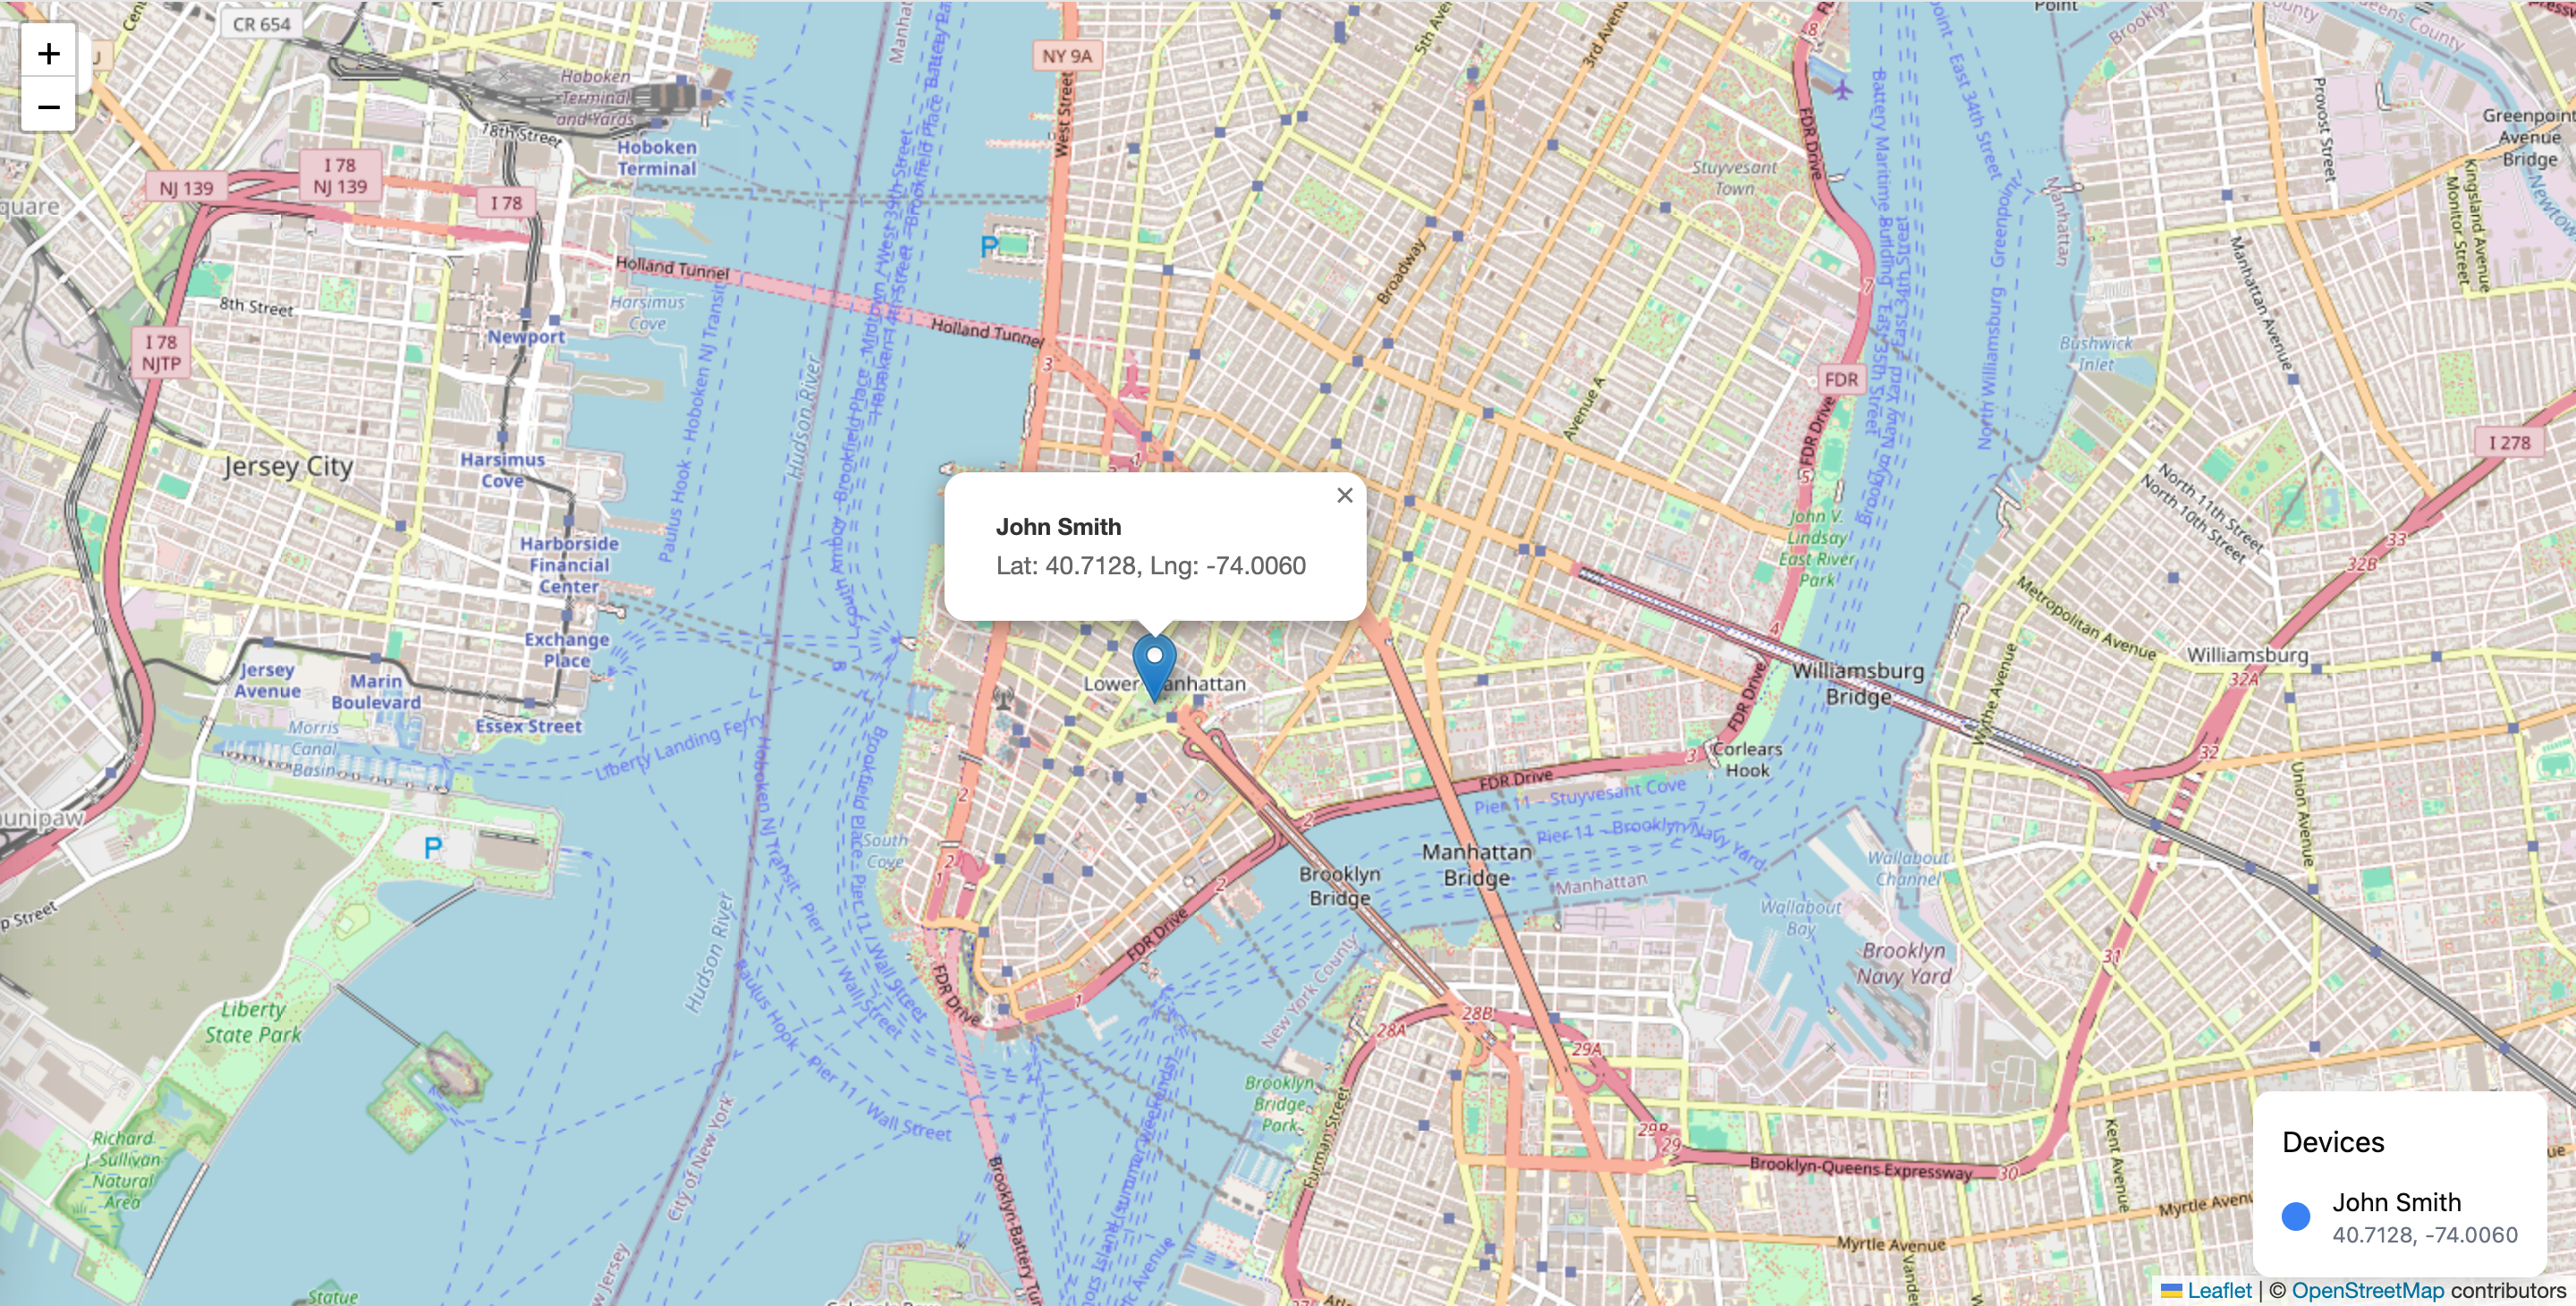
\includegraphics[width=0.75\textwidth]{png/screenshots/FigmaUISS.png}
    \caption{\FigureLabel{PaperPrototype}: Figma Paper Prototype for FindIt UI.}
    \label{fig:figmaUI}
    \vspace{1em}
\end{figure}

% ------------ Figure 2 --------------------
\begin{figure}[!htbp]
    \centering
    \vspace{1em}
    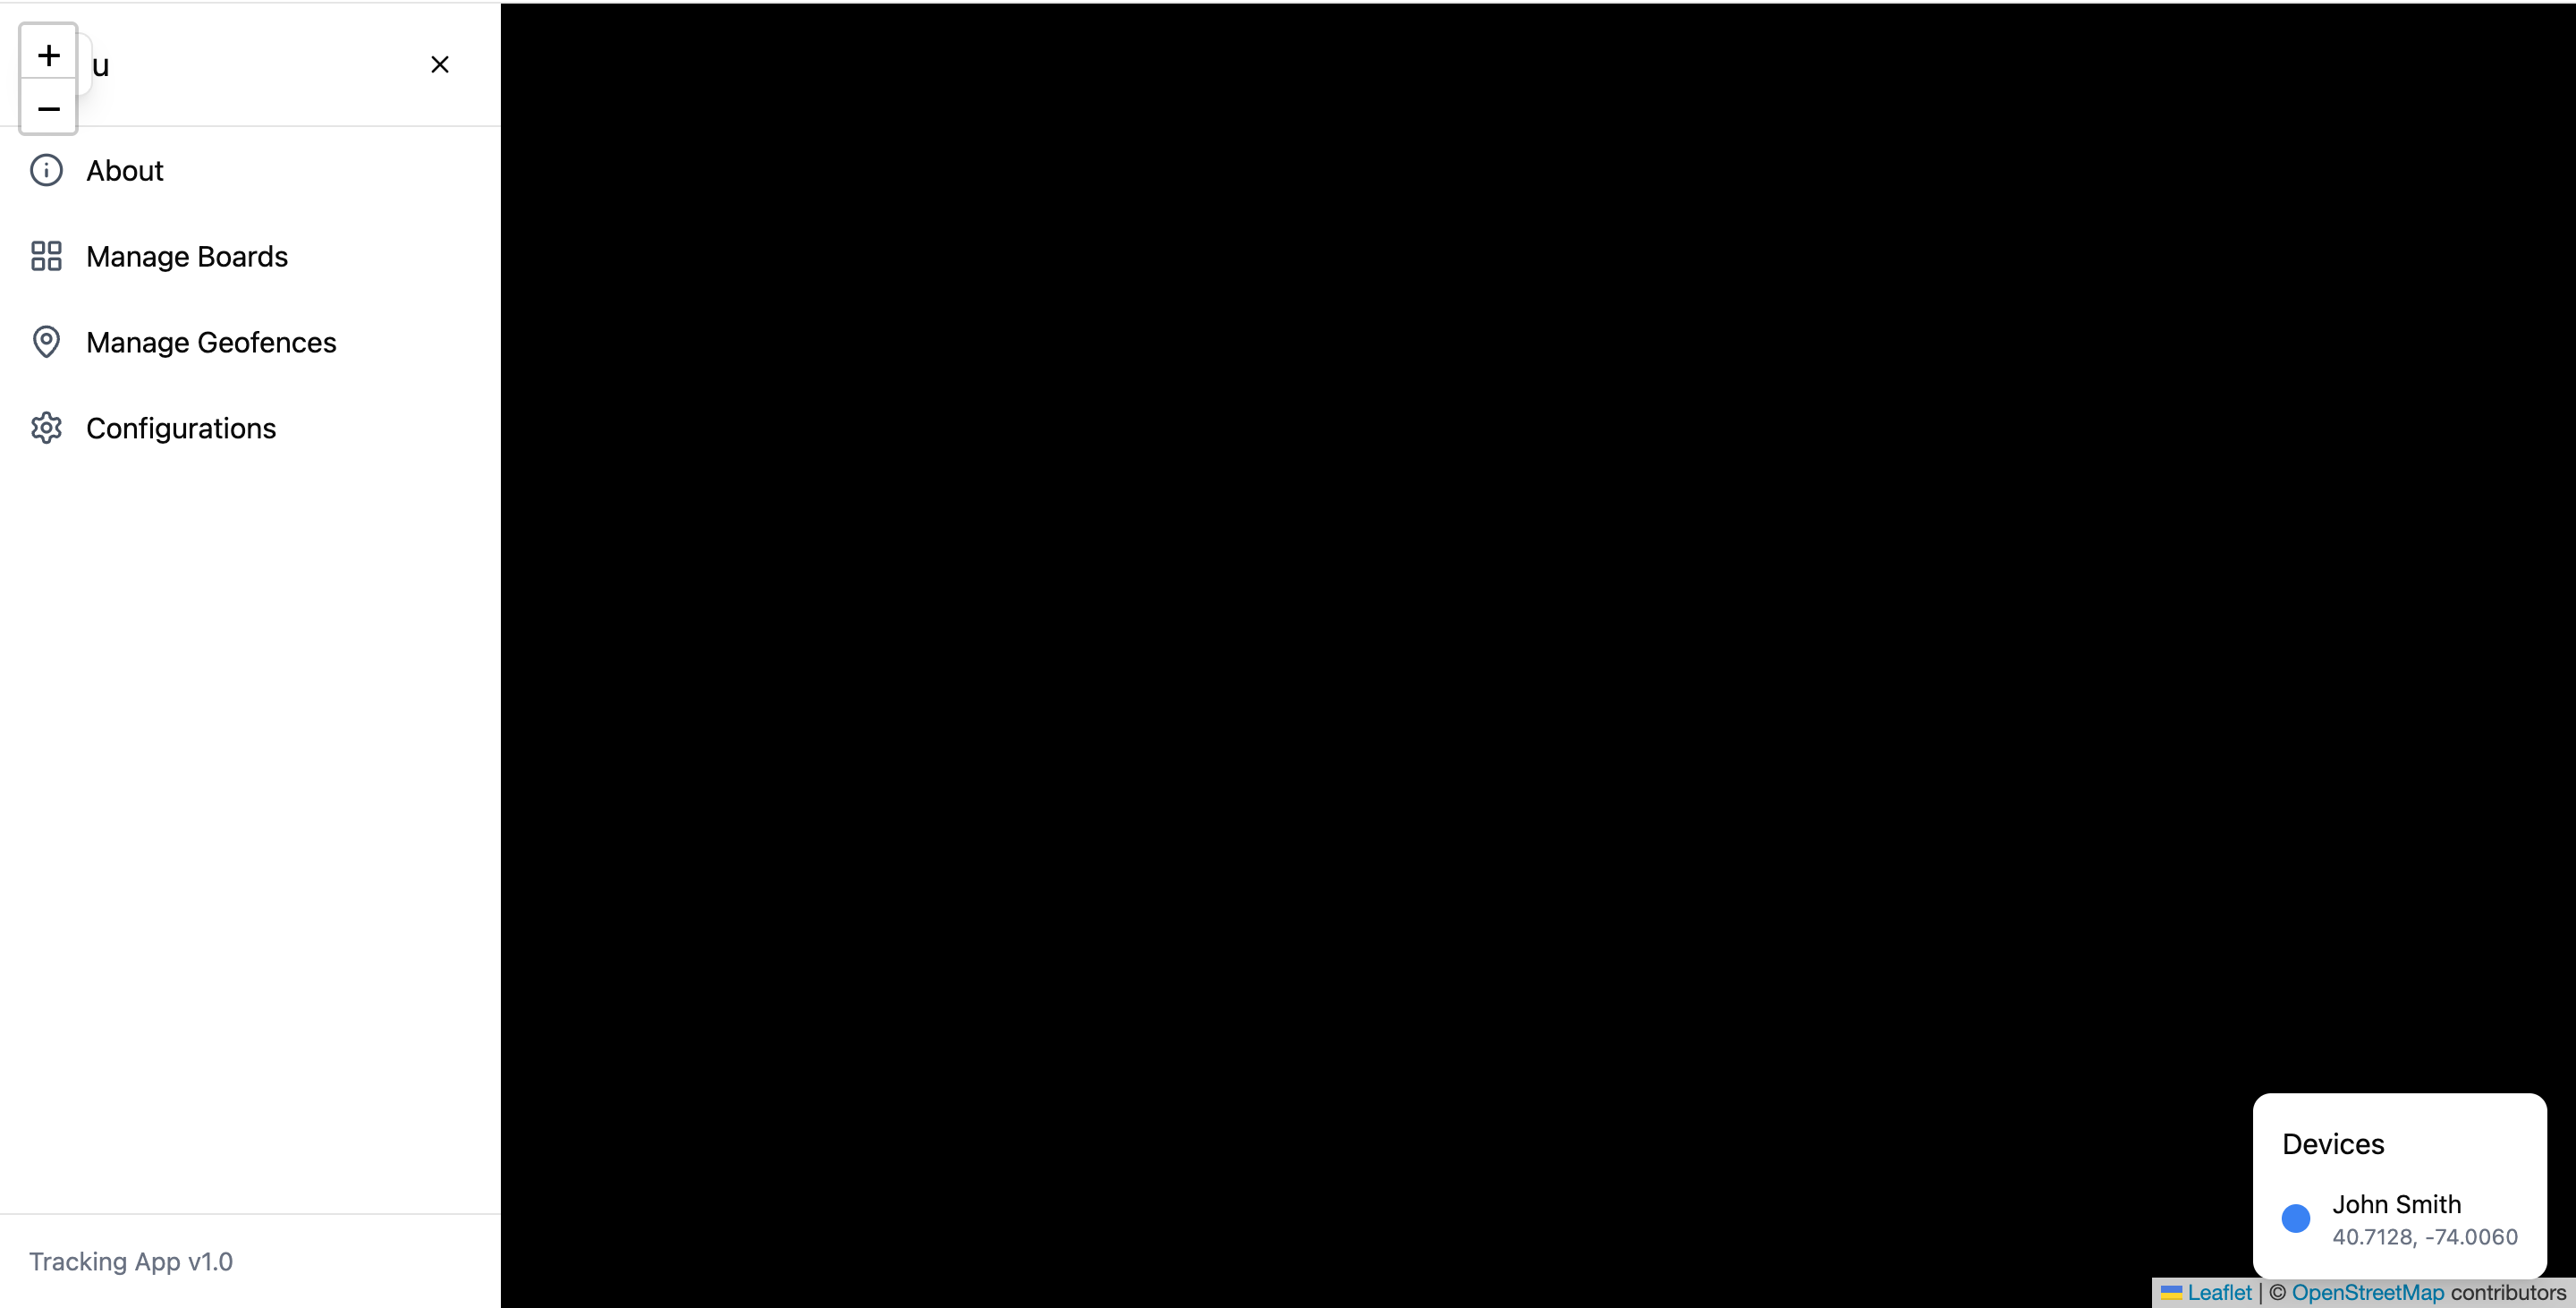
\includegraphics[width=0.75\textwidth]{png/screenshots/UISideMenu.png}
    \caption{\FigureLabel{PaperPrototype}: Figma Paper Prototype of Side Menu.}
    \label{fig:FigmaMenu}
    \vspace{1em}
\end{figure}

% ------------ Figure 3 --------------------
\begin{figure}[!htbp]
    \centering
    \vspace{1em}
    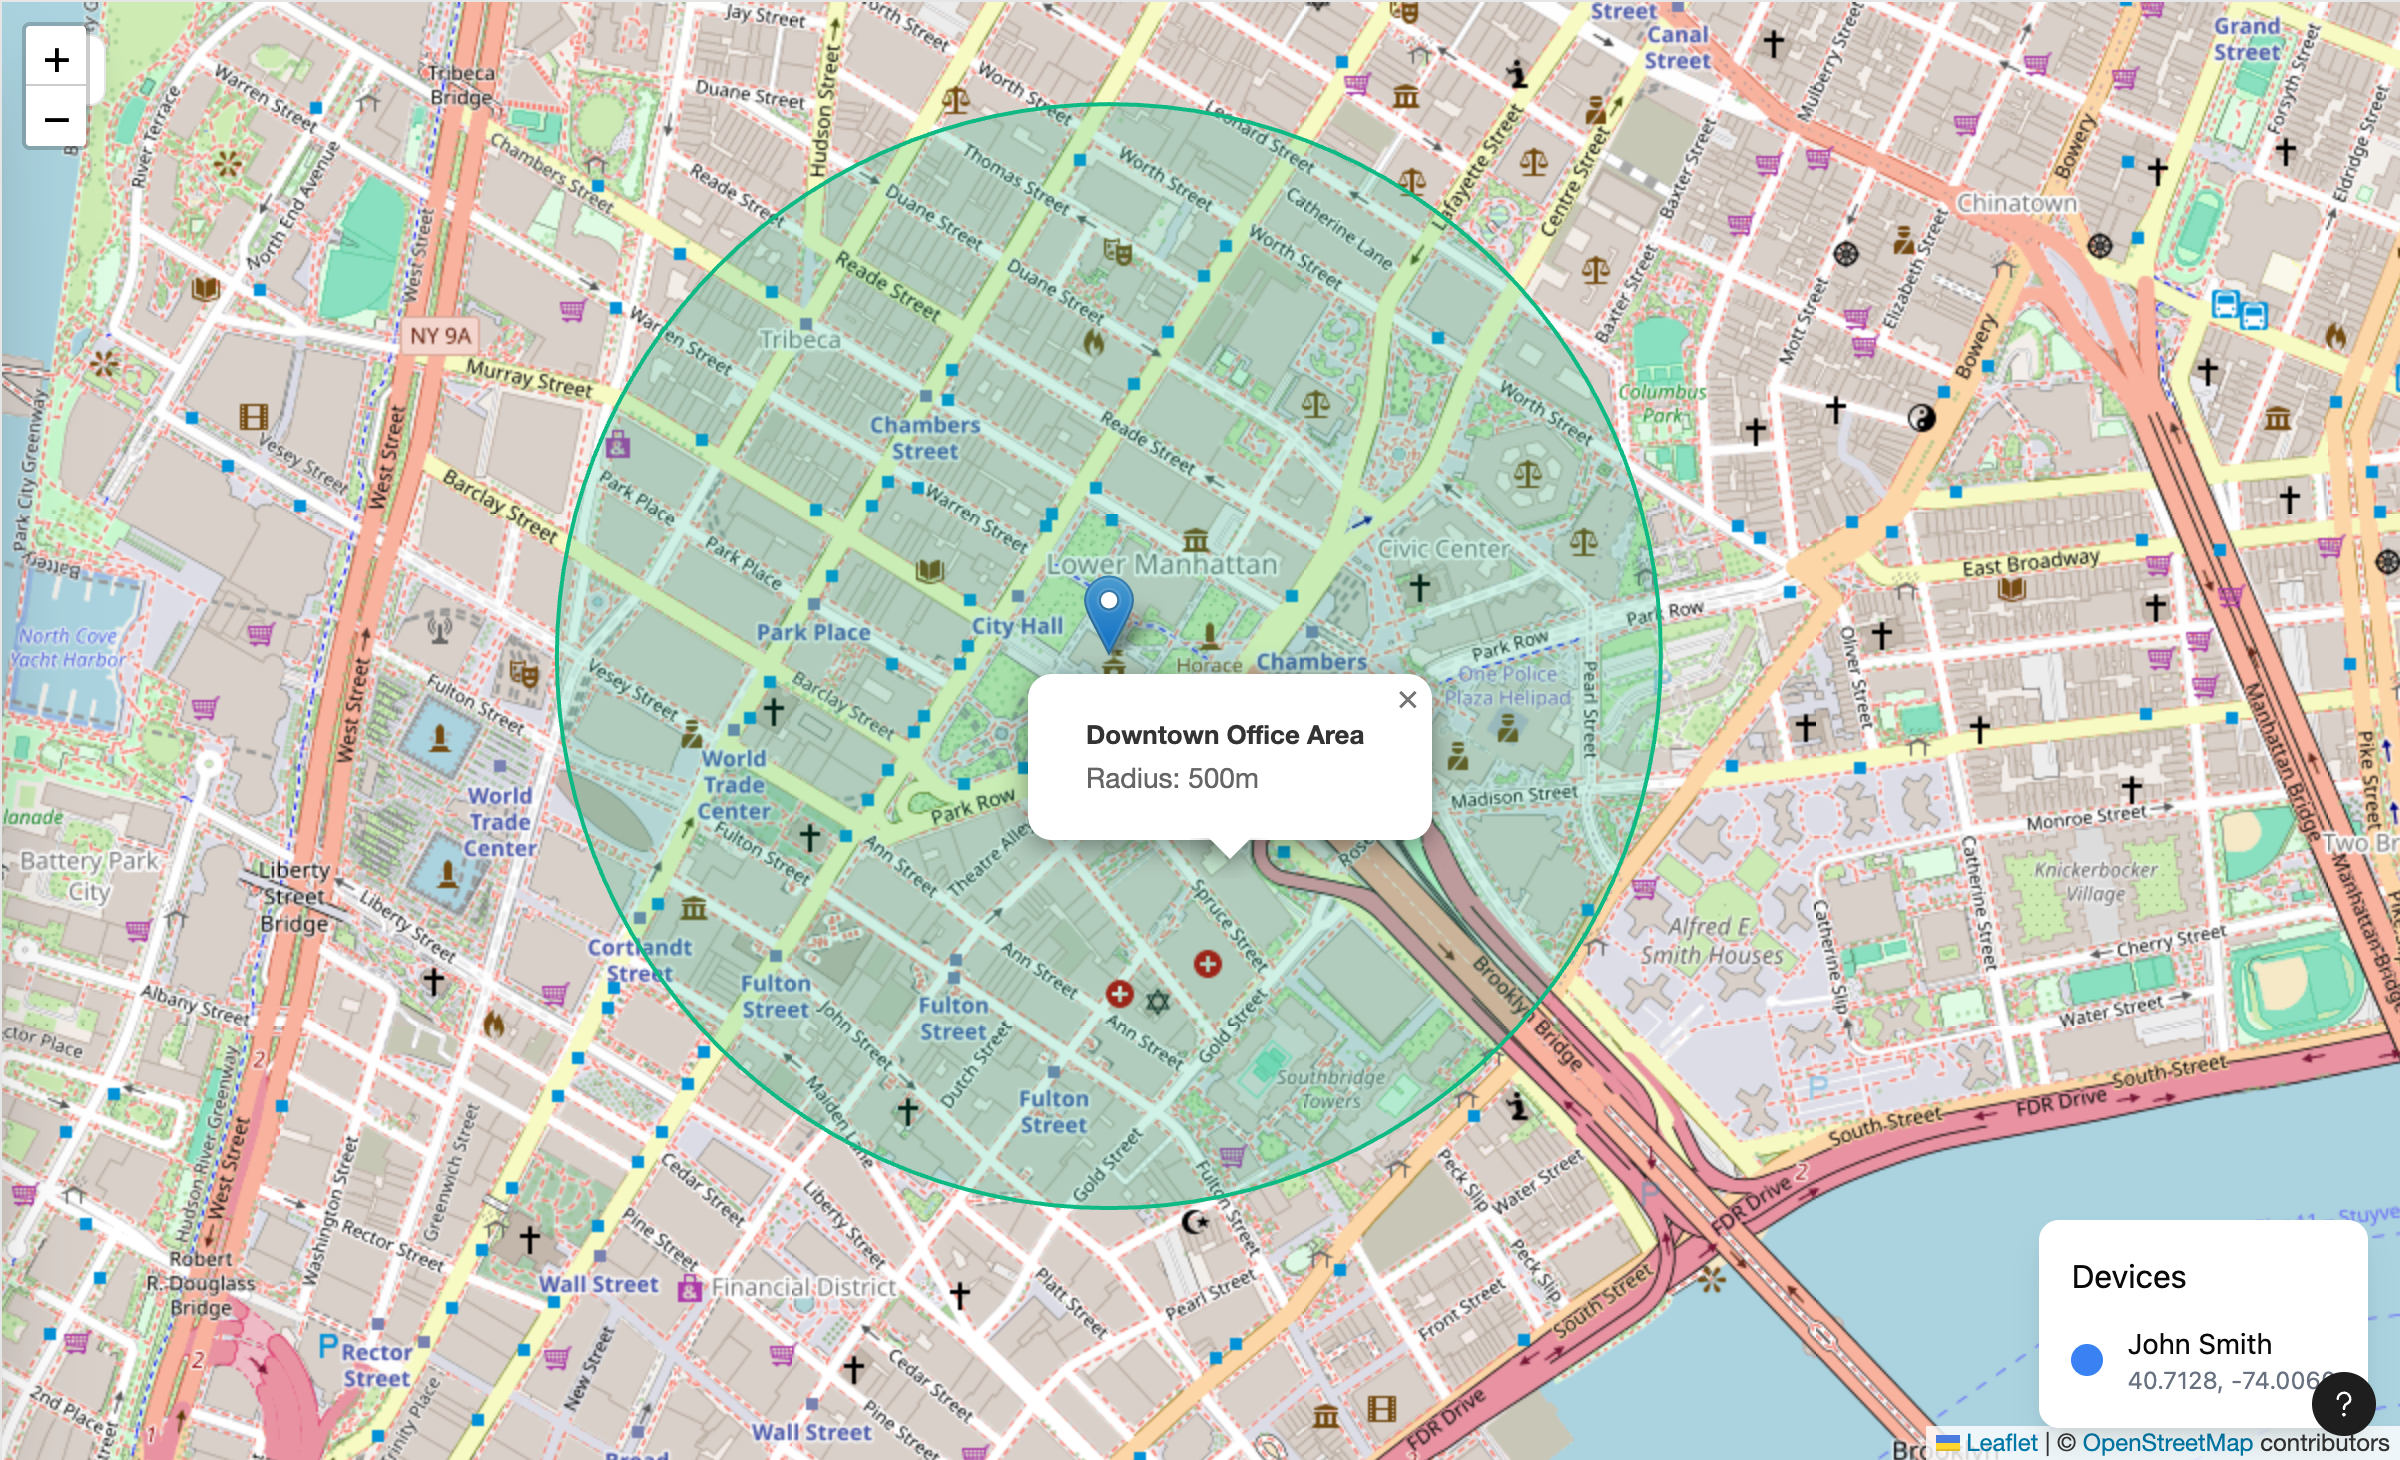
\includegraphics[width=0.75\textwidth]{png/screenshots/geofenceFigma.png}
    \caption{\FigureLabel{PaperPrototype}: Figma Paper Prototype of Geofence Implementation.}
    \label{fig:FigmaGeofence}
    \vspace{1em}
\end{figure}

\chapter{Logical View \\
\small{\textit{-- Ryan Davis, Roy Tas, and Cory Vitanza}}
\index{Logical View} 
\index{Chapter!Logical View}
\label{Chapter::LogicalView}}

Class diagrams present the structure of our Design, highlighting the firmware on our Wio Tracker 1110, and how that data is processed in our React software.
%class diagram good

\begin{figure}[h]
\centering

\includegraphics[width=0.7\textwidth]{png/diagrams/Firmware Class Diagram.jpg}
\caption{\FigureLabel{FirmwareClasses}: Class diagram for the Wio Tracker 1110 Development Board's Firmware}
\label{fig:FirmwareClasses}
\end{figure}

\begin{figure}[h]
\centering

\includegraphics[width=1.15\textwidth]{png/diagrams/ReactMVC.jpg}
\caption{\FigureLabel{Model View Controller}: Class Diagram for our React Interface Using the model view controller design pattern.}
\label{fig:MVCClasses}
\end{figure}

\section*{Class Diagram Description}

\begin{itemize}

    \item \textbf{Overview}
    \begin{itemize}
        \item The class diagram is organized into four major packages: \textbf{Entities}, \textbf{Models}, \textbf{Controllers}, and \textbf{Views}.
        \item This structure follows the Model--View--Controller (MVC) architectural pattern.
        \item Each package contains classes with specific responsibilities and well-defined relationships such as inheritance, composition, realization, and dependencies.
    \end{itemize}

    \item \textbf{Entities Package}
    \begin{itemize}
        \item Contains raw data structures corresponding to the Supabase database tables.
        \item Includes \texttt{BoardEntity}, \texttt{GeofenceEntity}, \texttt{AccountEntity}, and \texttt{LocationRecordEntity}.
        \item All entities implement the \texttt{IEntity} interface, which standardizes the attribute \texttt{id} across all stored records.
        \item Entities contain no domain logic and only represent database rows.
    \end{itemize}

    \item \textbf{Models Package}
    \begin{itemize}
        \item Models wrap the Entities through composition and extend the abstract \texttt{Model} base class.
        \item Responsible for data cleaning, validation, and transformation (e.g., converting timestamps to \texttt{Date} objects).
        \item Contain computed attributes required by the UI, such as geofence containment, distance calculations, battery warnings, and formatted display information.
        \item Includes \texttt{BoardModel}, \texttt{GeofenceModel}, \texttt{AccountModel}, and \texttt{LocationRecordModel}.
    \end{itemize}

    \item \textbf{Controllers Package}
    \begin{itemize}
        \item All controllers implement the \texttt{Controller} interface.
        \item Responsible for orchestrating system logic, including loading database data, updating models, applying filters, and managing CRUD operations.
        \item Controllers detect events such as geofence breaches or location abnormalities, and trigger notifications via \texttt{NotificationService}.
        \item Includes \texttt{BoardController}, \texttt{GeofenceController}, \texttt{FilteringController}, and \texttt{NotificationController}.
    \end{itemize}

    \item \textbf{Views Package}
    \begin{itemize}
        \item Views depend on their corresponding controller to retrieve and update models.
        \item Views do not contain domain logic---their only responsibility is UI rendering.
        \item Views interact with the \texttt{MapComponent} to display board locations, geofences, filters, and violations.
        \item Includes \texttt{BoardView}, \texttt{GeofenceView}, \texttt{AccountView}, and the shared \texttt{MapComponent}.
    \end{itemize}

    \item \textbf{Key Relationships}
    \begin{itemize}
        \item \textbf{Inheritance:}
        \begin{itemize}
            \item Model subclasses extend the abstract \texttt{Model}.
            \item Controllers implement \texttt{IController}.
            \item Views depend on \texttt{MapView}.
        \end{itemize}
        \item \textbf{Composition:}
        \begin{itemize}
            \item Each Model class owns its corresponding Entity (e.g., \texttt{BoardModel} has a \texttt{BoardEntity}).
        \end{itemize}
        \item \textbf{Dependencies:}
        \begin{itemize}
            \item Views depend on Controllers.
            \item Controllers depend on Models and backend API calls.
            \item Views depend on the shared \texttt{MapComponent} for UI rendering.
        \end{itemize}
        \item \textbf{Separation of Concerns:}
        \begin{itemize}
            \item Views never access Entities or perform domain logic.
            \item Models never render UI.
            \item Controllers manage logic but never render UI directly.
        \end{itemize}
    \end{itemize}

    \item \textbf{Summary}
    \begin{itemize}
        \item The diagram demonstrates a complete and maintainable MVC architecture.
        \item Entities represent raw data, Models transform and prepare information for use, Controllers coordinate and implement CRUD, and Views render the user-facing interface.
        \item This architecture supports geofence and board management, filtering operations, map visualization, and notification handling in the FindIt system.
    \end{itemize}

\end{itemize}

\chapter{Development View \\
\small{\textit{-- Ryan Davis, Roy Tas, and Cory Vitanza}}
\index{Development View} 
\index{Chapter!DevelopmentView}
\label{Chapter::DevelopmentView}}

The package diagram for the FindIt system highlights the different modules in our system. The Wio Tracker 1110 has firmware, uplinking the data it collected into the database. The database provides data to our ML model highlighting abnormalities in location data, and to the React frontend, where the data is processed and presented on the user interface.
%Package Diagram

\begin{figure}[h]
\centering
\includegraphics[width=0.7\textwidth]{png/diagrams/FindIt Package Diagram.jpg}
\caption{\FigureLabel{Package Diagram}: Package diagram for FindIt deployment}
\label{fig:packageDiagram}
\end{figure}
\chapter{Process View \\
\small{\textit{-- Ryan Davis, Roy Tas, and Cory Vitanza}}
\index{Process View} 
\index{Chapter!ProcessView}
\label{Chapter::ProcessView}}

This sequence diagram shows the flows for our most prevalent use case, multi-resident monitoring. The activity starts with boards collecting gps data, and provides the end user with location data and notifications if a board leaves the geofence.

%Sequence Diagram
\begin{figure}[h]
\centering
\includegraphics[width=0.7\textwidth]{png/diagrams/UC2-Activity.png}
\caption{\FigureLabel{ucMultiResidentMonitoringActivity}: Activity Diagram for Multi-Resident Monitoring \hyperref[UseCaseTable2]{(UC2)}}
\label{fig:ucMultiResidentMonitoringActivity}
\end{figure}


\chapter{Physical View \\
\small{\textit{-- Ryan Davis, Roy Tas, and Cory Vitanza}}
\index{physical view} 
\index{Chapter!PhysicalView}
\label{Chapter::PhysicalView}}

FindIt component diagram depicting the interfaces for the different components of the system, including the development board, database, backend infrastructure, and react components.

%Component Diagram
\begin{figure}[h]
\centering

\includegraphics[width=\textwidth]{png/diagrams/FindIt Component Diagram.jpg}
\caption{\FigureLabel{Component Diagram}: Component diagram for FindIt deployment}
\label{fig:componentDiagram}
\end{figure}
\chapter{Preliminary Implementation Report \\
\small{\textit{-- Ryan Davis, Roy Tas, and Cory Vitanza}}
\index{Preliminary Implementation Replrt} 
\index{Chapter!PreliminaryImplementation}
\label{Chapter::PreliminaryImplementation}}



% ---------- Glossary ----------
\cleardoublepage
\phantomsection
\glsaddall
\printnoidxglossaries
\label{Chapter::Glossary}

% ---------- Appendices ----------
\appendix
\chapter{Weekly Reports \\
\small{\textit{- Ryan Davis, Cory Vitanza, and Roy Tas}}%
}
\index{weekly reports}
\index{Chapter!Weekly Reports}
\label{Chapter::WeeklyReports}

%=======================================================
\section{Week Report 13 (12/11/2025)}
\label{sec:report13}

\subsection{Progress Made}
\begin{itemize}

    \item Connected board to SenseCraft UI for GPS testing.

    \begin{figure}[H]
        \centering
        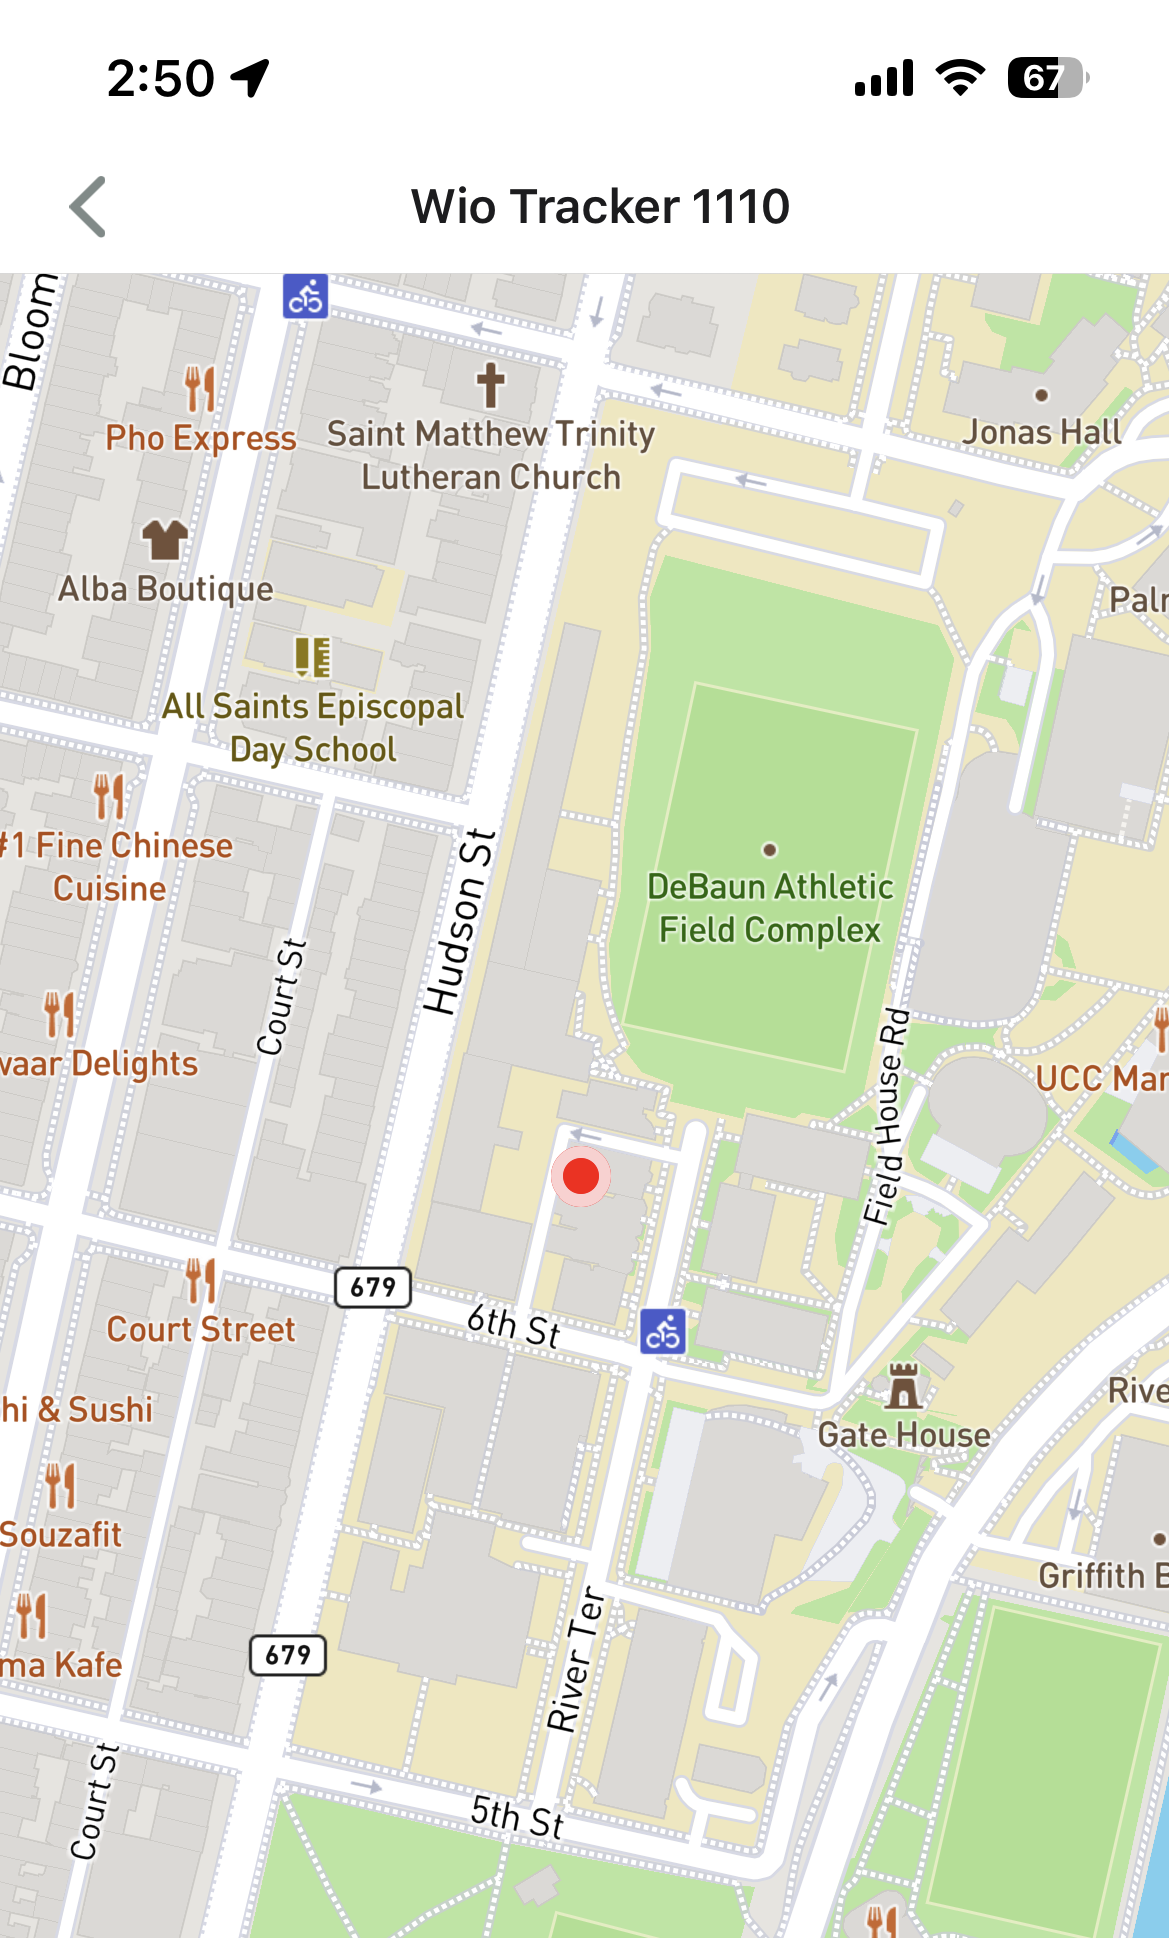
\includegraphics[width=0.7\textwidth]{png/screenshots/sensecraft.png}
        \caption{\FigureLabel{SensecraftConnection}: SenseCraft UI connection for GPS testing}
        \label{fig:SensecraftConnection}
    \end{figure}
    The screenshot above shows the device’s GPS output appearing correctly in SenseCraft.

    \item Developed authorization protocol with React Frontend and Supabase Database for user accounts.
    % Uncomment when screenshot ready:
    \begin{figure}[H]
        \centering
        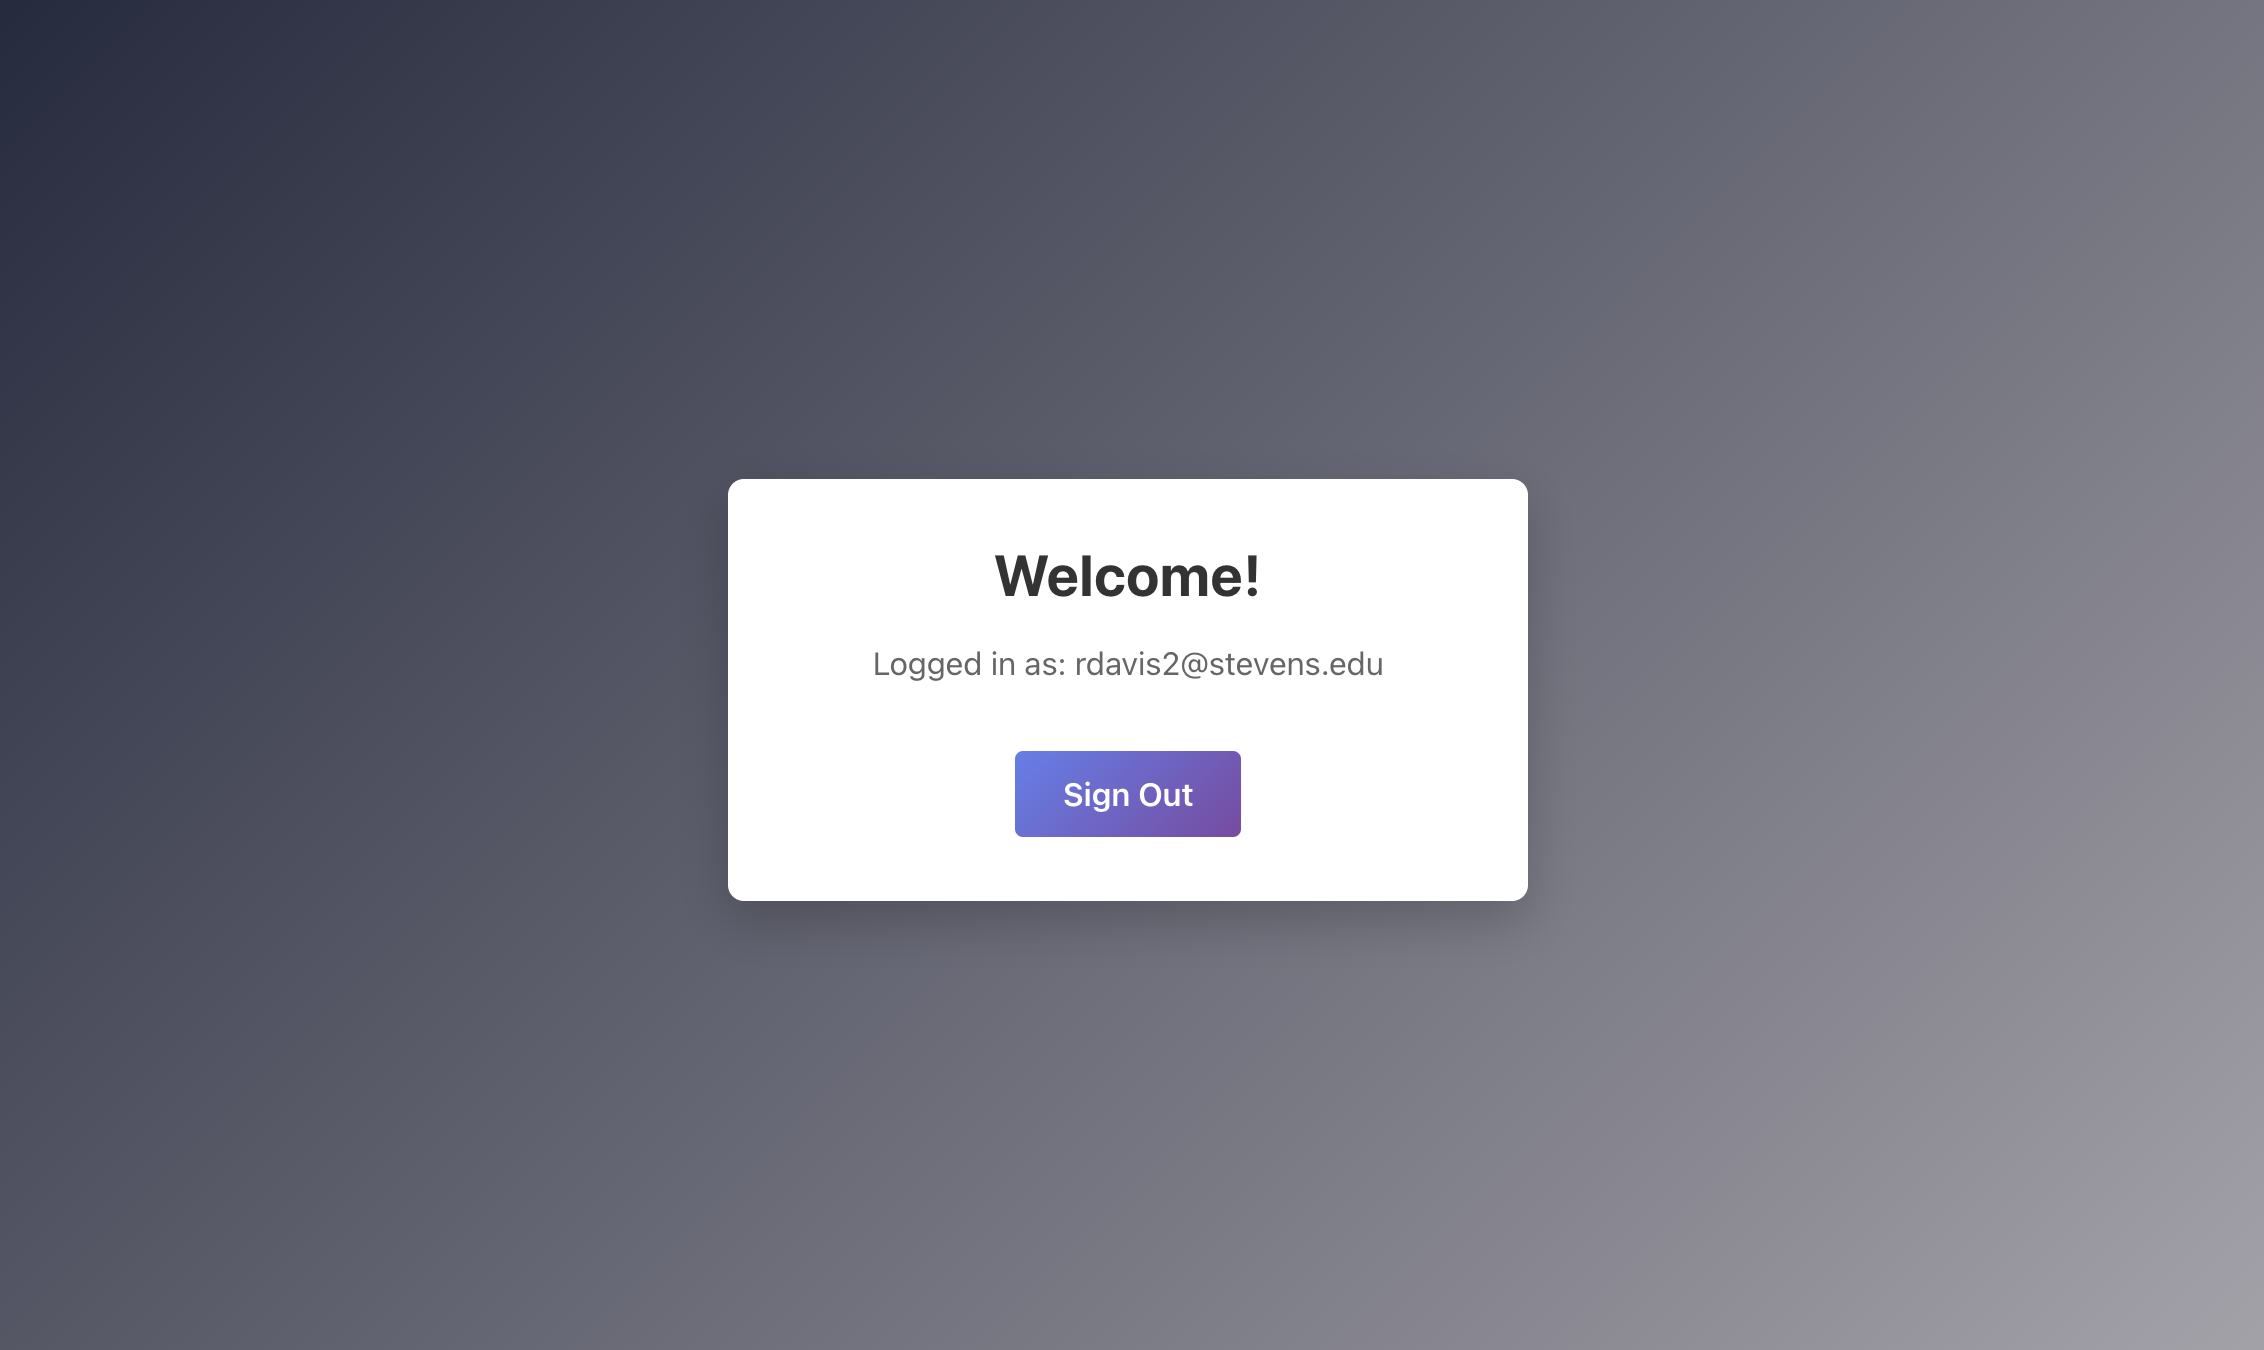
\includegraphics[width=0.7\textwidth]{png/screenshots/AuthUI.png}
        \caption{\FigureLabel{DevServer}: React development server showing authorization flow}
        \label{fig:DevServer}
    \end{figure}
    The figure above would show the login system functioning in the dev server.

    \item Established database schema for board integrations.

    \begin{figure}[H]
        \centering
        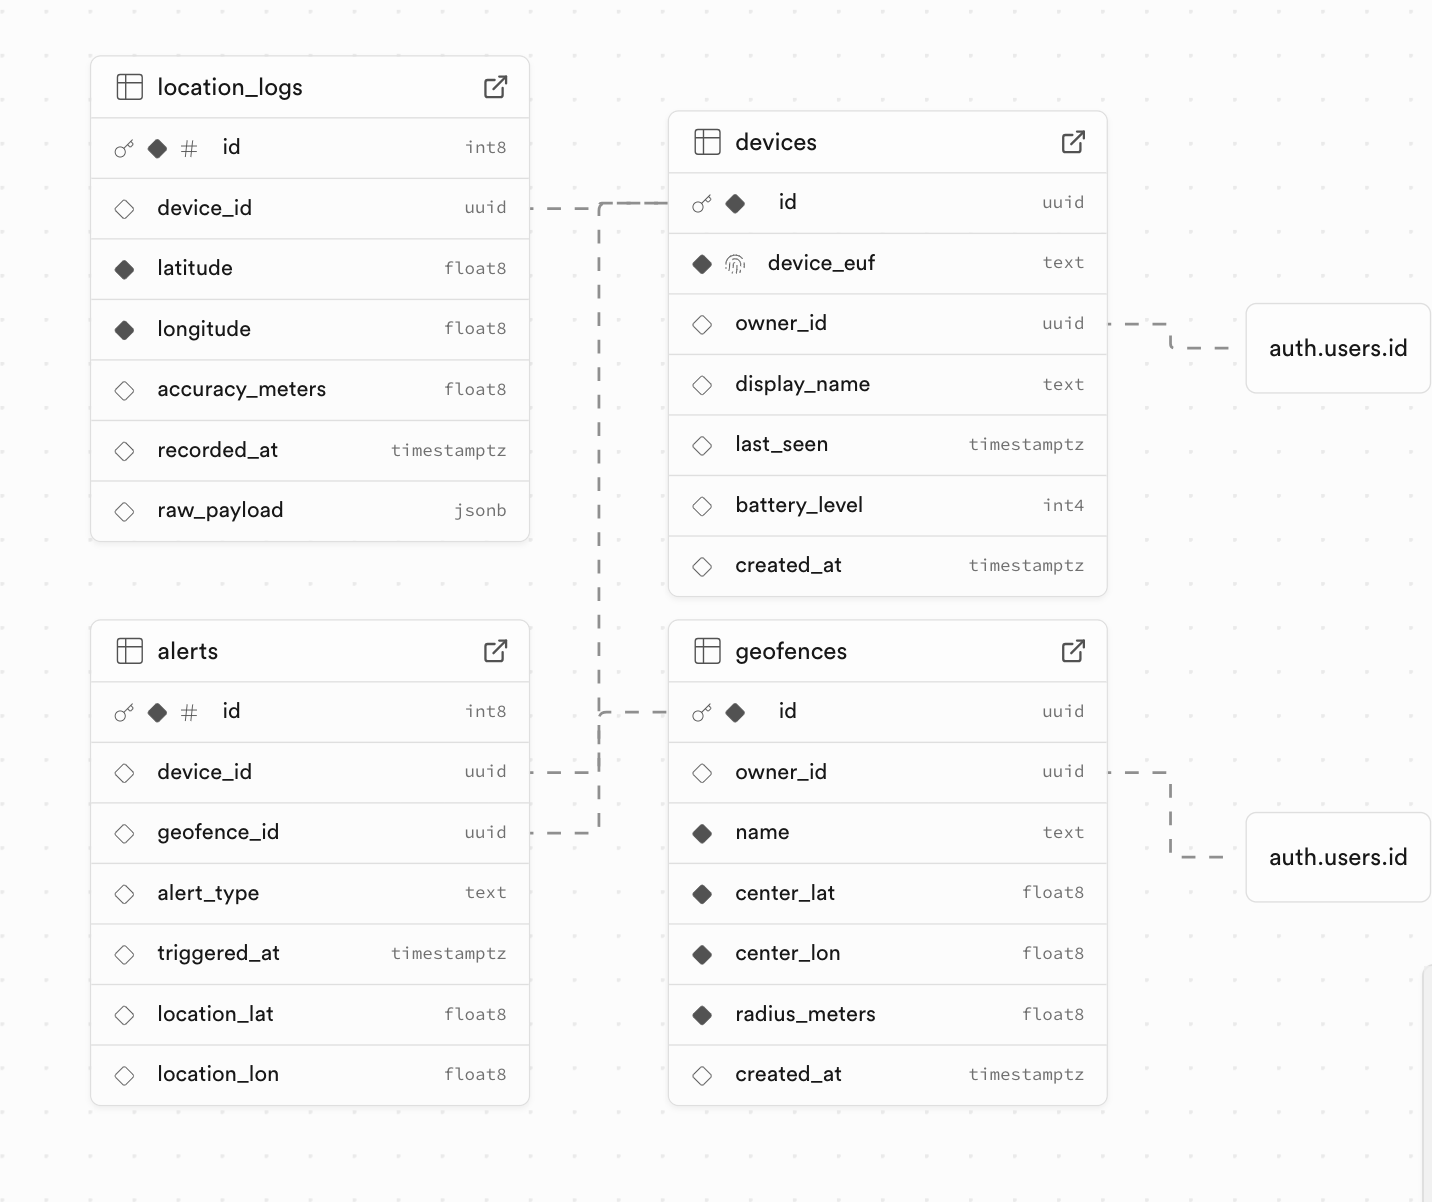
\includegraphics[width=0.7\textwidth]{png/screenshots/dbSchema.png}
        \caption{\FigureLabel{SupabaseSchema}: Supabase schema for board integration}
        \label{fig:SupabaseSchema}
    \end{figure}
    The schema diagram above shows how each device is linked to a user via \texttt{auth.users.id}.

    \item Developed a case for the Wio Tracker 1110.

    \begin{figure}[H]
        \centering
        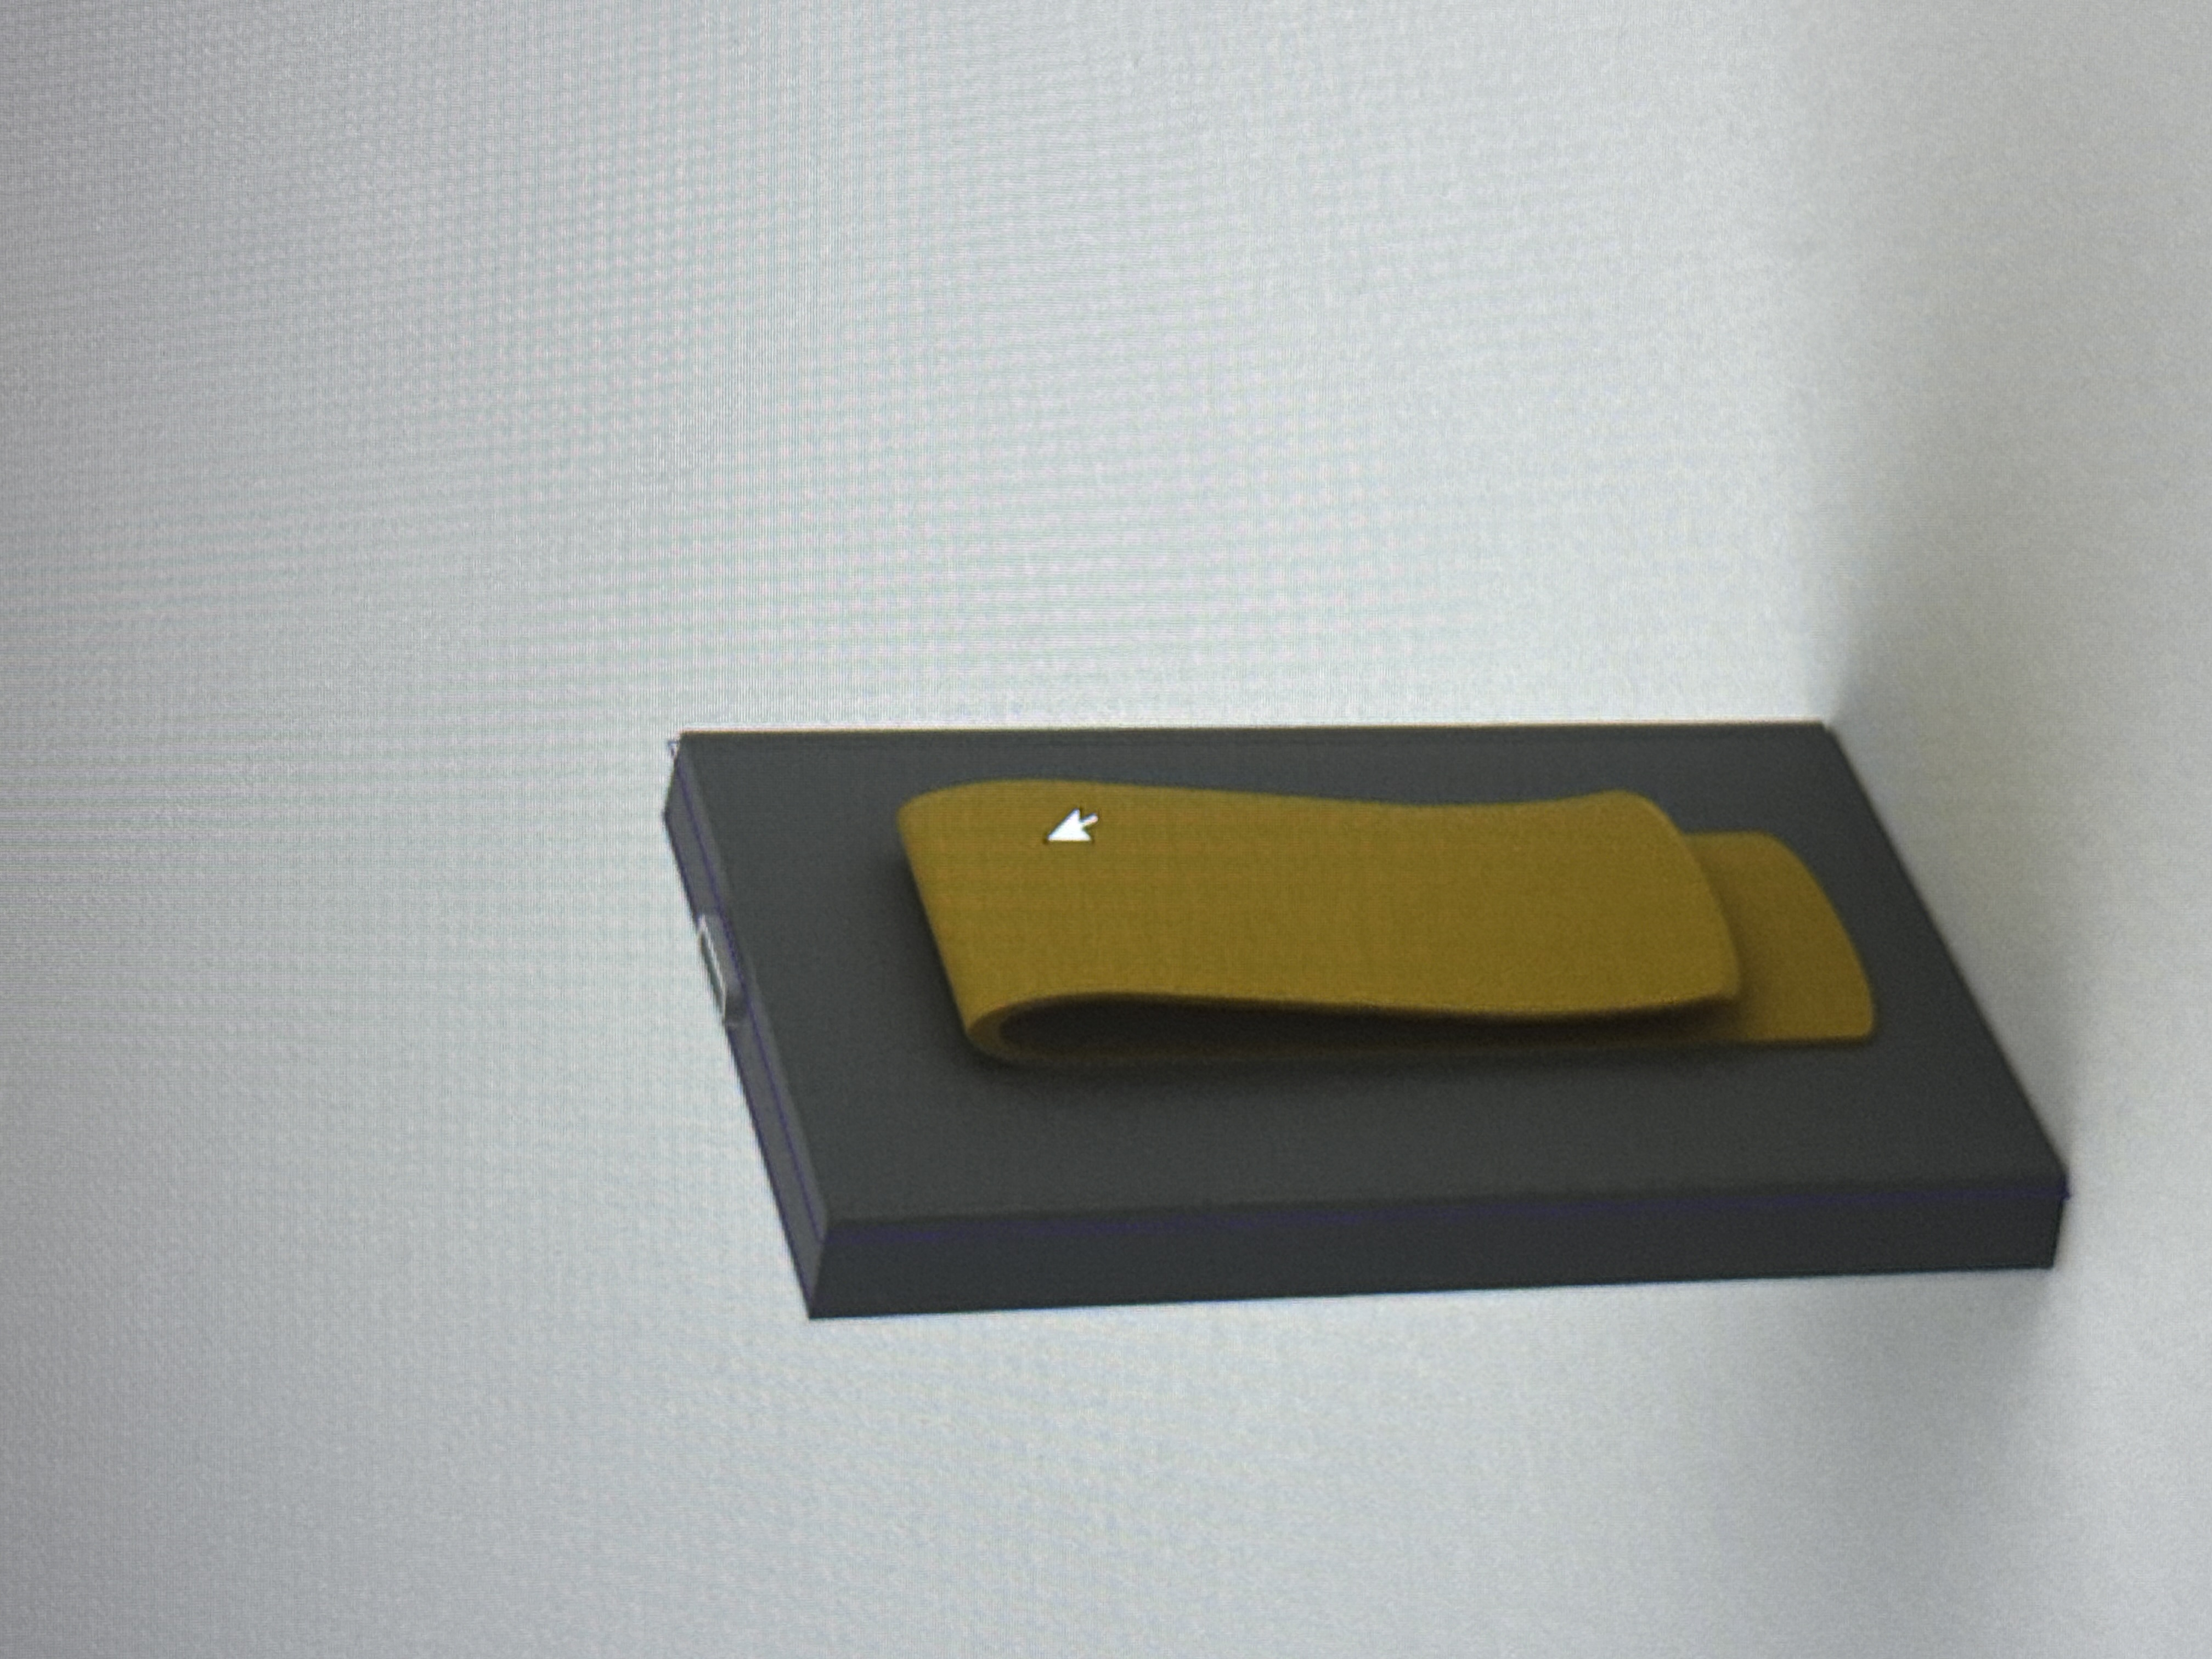
\includegraphics[width=0.7\textwidth]{png/screenshots/caseClip.png}
        \caption{\FigureLabel{CaseClip}: Clip for the Wio Tracker 1110}
        \label{fig:CaseClip}
    \end{figure}
    The clip design above demonstrates the mounting mechanism for the tracker.

    \begin{figure}[H]
        \centering
        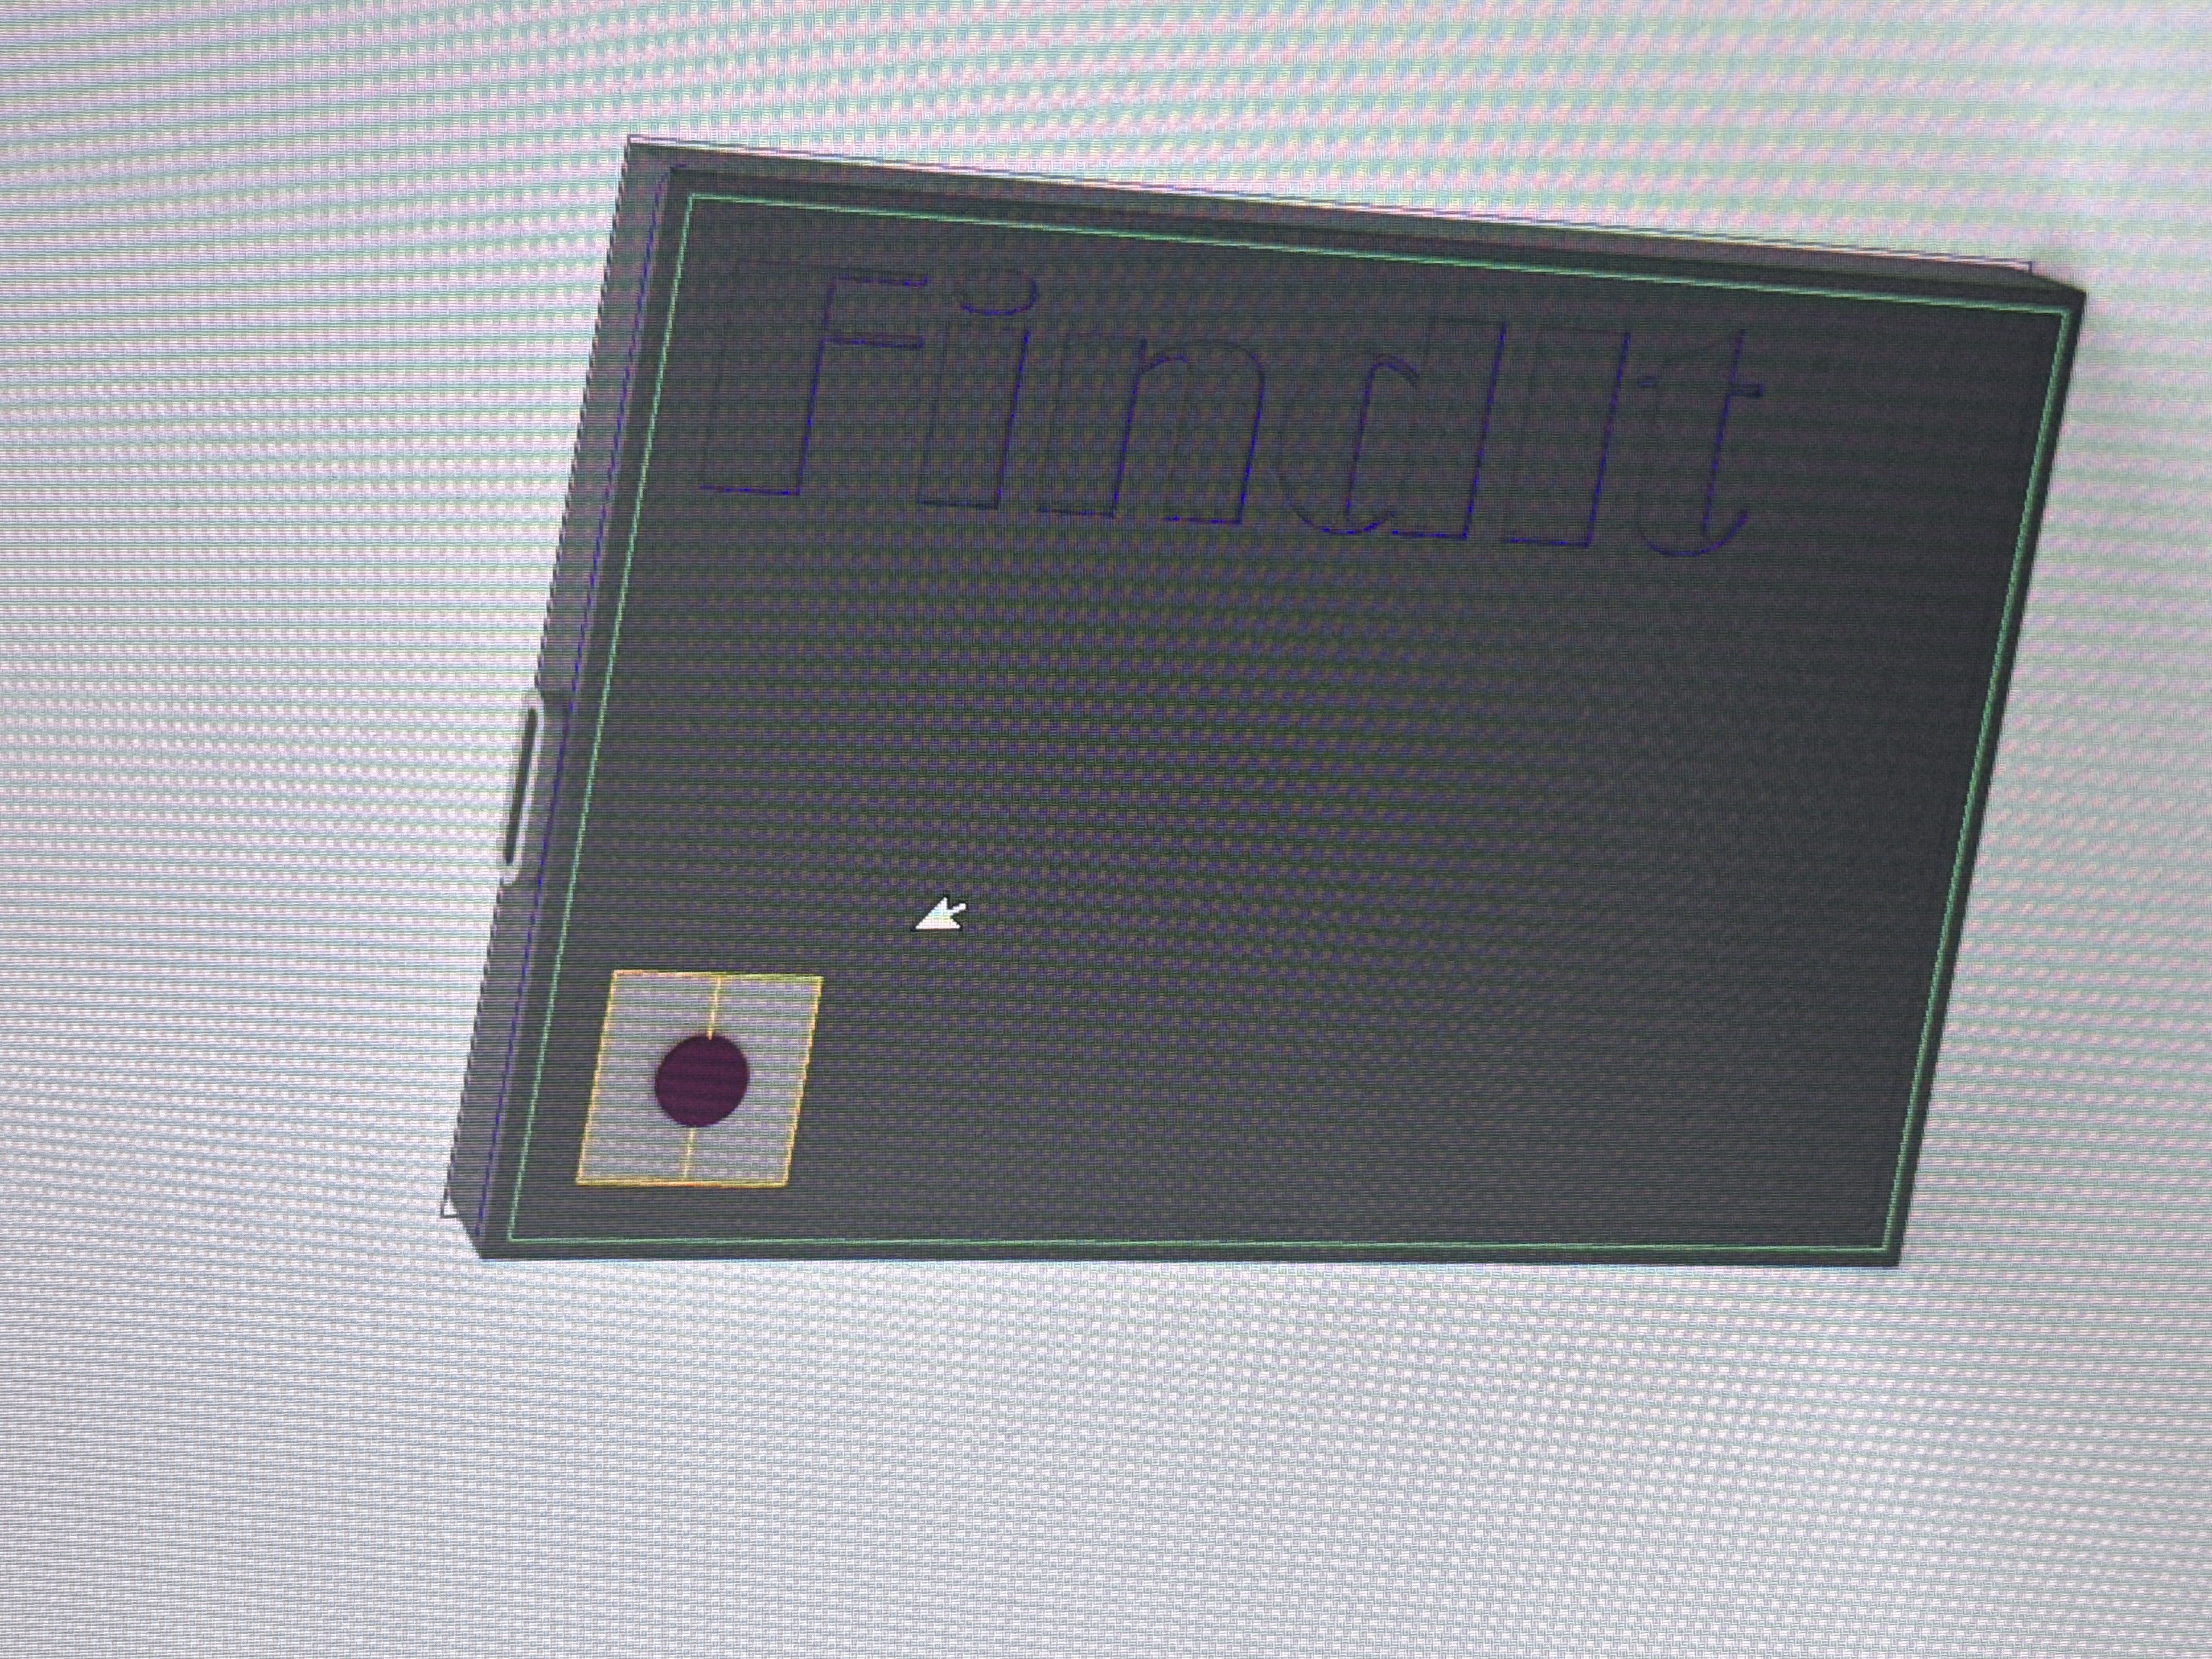
\includegraphics[width=0.7\textwidth]{png/screenshots/caseIsometric.png}
        \caption{\FigureLabel{CaseIsometric}: Isometric view of the initial case prototype}
        \label{fig:CaseIsometric}
    \end{figure}
    The isometric view above provides a full perspective of the initial enclosure prototype.

    \item Flashed board with default firmware to connect to SenseCraft UI and retrieve LoRaWAN device keys.
    % Uncomment when screenshot ready:
    %\begin{figure}[H]
    %    \centering
    %    \includegraphics[width=0.7\textwidth]{png/screenshots/serial_output.png}
    %    \caption{\FigureLabel{SerialOutput}: Serial monitor output during firmware flashing}
    %    \label{fig:SerialOutput}
    %\end{figure}
    %Serial output screenshot would appear here.

\end{itemize}

\subsection{Next Week's Plan}
\begin{itemize}
    \item Continue configuring the board to connect to the LoRaWAN network server.
    \item Implement OpenStreetMaps API in the React frontend for mapping functionality.
\end{itemize}


%=======================================================
\section{Week Report 12 (12/05/2025)}
\label{sec:report12}

\subsection{Progress Made}
\begin{itemize}
    \item Received the Wio Tracker 1110 Development Board.
    \item Configured The Things Stack LoRaWAN network.
    \item Initialized database tables and schema.
\end{itemize}

\subsection{Next Week's Plan}
\begin{itemize}
    \item Configure the development board with SenseCap to collect device keys.
    \item Debug the firmware to optimize GPS collection and confirm LoRaWAN uplinks.
    \item Prepare the React user interface for prototype demonstration.
\end{itemize}


%=======================================================
\section{Week Report 11 (11/14/2025)}
\label{sec:report11}

\subsection{Progress Made}
\begin{itemize}
    \item Created a \hyperref[fig:figmaUI]{Paper Prototype} for the FindIt user interface.
    \item Developed user personas for the \hyperref[Chapter::UserInterfaceDesign]{User Interface Design}.
    \item Began composing UML diagrams for the \hyperref[Chapter::LogicalView]{logical view} (class diagram), \hyperref[Chapter::DevelopmentView]{development view} (component diagram), \hyperref[Chapter::ProcessView]{process view} (sequence diagram), and \hyperref[Chapter::PhysicalView]{physical view} (package diagram).
\end{itemize}

\subsection{Next Week's Plan}
\begin{itemize}
    \item Begin firmware development for the Wio Tracker 1110.
    \item Finalize UML diagrams for all system views.
\end{itemize}


%=======================================================
\section{Week Report 10 (11/7/2025)}
\label{sec:report10}

\subsection{Progress Made}
\begin{itemize}
    \item Initialized The Things Stack LoRaWAN network in preparation for the development board.
    \item Reordered the board from a different vendor to reduce wait times.
\end{itemize}

\subsection{Next Week's Plan}
\begin{itemize}
    \item Begin work on Preliminary Design: User personas, UI design, Architecture, Use Cases, Logical view, Development view, Process view, Physical view.
    \item Continue developing the frontend regardless of board arrival.
    \item Collect board measurements to design the device case.
\end{itemize}


%=======================================================
\section{Week Report 9 (10/31/2025)}
\label{sec:report9}

\subsection{Progress Made}
\begin{itemize}
    \item Created \hyperref[section::activityDiagrams]{activity diagrams} for all six use cases.
    \item Initialized The Things Stack LoRaWAN server in preparation for the development board.
\end{itemize}

\subsection{Next Week's Plan}
\begin{itemize}
    \item Refine requirements and use cases.
    \item Create system classes that correspond to activity diagrams.
\end{itemize}


%=======================================================
\section{Week Report 8 (10/24/2025)}
\label{sec:report8}

\subsection{Progress Made}
\begin{itemize}
    \item Initialized infrastructure: Supabase database, React frontend, Postman API testing environment, and CI pipeline.
    \item Populated Kanban board for development tasks.
    \item Added more activity diagrams to reflect system behaviors.
\end{itemize}

\subsection{Next Week's Plan}
\begin{itemize}
    \item Begin UI construction and GPS coordinate testing.
    \item Finalize requirements, use cases, and user stories.
    \item Prepare and present the Project Concept Development and Specification Demo.
\end{itemize}


%=======================================================
\section{Week Report 7 (10/17/2025)}
\label{sec:report7}

\subsection{Progress Made}
\begin{itemize}
    \item Created \hyperref[fig:finditUseCases]{Use Case Diagram} for the FindIt system.
    \item Created \hyperref[fig:finditActivity1]{Activity Diagram}.
    \item Completed budget update to order the Wio Tracker 1110 development board.
\end{itemize}

\subsection{Next Week's Plan}
\begin{itemize}
    \item Begin Arduino firmware development (pending board arrival).
    \item Begin setting up CI/CD infrastructure and Supabase database.
\end{itemize}


%=======================================================
\section{Week Report 6 (10/10/2025)}
\label{sec:report6}

\subsection{Progress Made}
\begin{itemize}
    \item Updated \hyperref[Chapter::Requirements]{Requirements} chapter.
    \item Added \hyperref[Chapter::UseCases]{Use Cases} chapter.
    \item Added \hyperref[Chapter::UserStories]{User Stories} chapter.
    \item Added \hyperref[Chapter::Glossary]{Glossary} chapter.
    \item Updated budget for new development board.
\end{itemize}

\subsection{Next Week's Plan}
\begin{itemize}
    \item Develop system UML diagrams.
    \item Meet with Dr. Damiano Zanotto.
    \item Continue building CI/CD infrastructure and Supabase.
    \item Await and debug new development board.
\end{itemize}


%=======================================================
\section{Week Report 5 (10/02/2025)}
\label{sec:report5}

\subsection{Progress Made}
This week, the team completed and presented our Demo for Project Mission and Development Plan. We set up our GitHub repository and created a project Kanban board to track tasks in an Agile workflow.

\subsection{Next Week's Plan}
Next week, we plan to order the new development board, begin frontend development, configure the Supabase backend, integrate CircleCI, and build our DevOps infrastructure.


%=======================================================
\section{Week Report 4 (09/25/2025)}
\label{sec:report4}

\subsection{Progress Made}
Our team determined that our current board (incorrect bootloader, XIAO preset) must be replaced with a proper Wio Tracker 1110 to regain full access to GPS, LoRa, and serial interfaces.

\subsection{Next Week's Plan}
We plan to complete Presentation 1, acquire the new board, set up GitHub + Agile boards, and begin GPS and data pipeline development.

\subsection{Risk Mitigation}
We aim to reduce the risk of inaccurate GPS tracking by implementing both indoor and outdoor tracking strategies.


%=======================================================
\section{Week Report 3 (09/18/2025)}
\label{sec:report3}

\subsection{Progress Made}
The team completed the \hyperref[Chapter::TeamDeclaration]{Team Declaration}, defining mission, drivers, and constraints.

\subsection{Next Week's Plan}
We will debug the Seeed LoRaWAN Arduino device: bootloader, buttons, GPS, LoRa module, and serial interface.

\subsection{Risk Mitigation}
The biggest risk is the malfunctioning Seeed LoRaWAN device. Mitigation includes testing alternative hardware such as the Raspberry Pi Nano.


%=======================================================
\section{Week Report 2 (09/12/2025)}
\label{sec:report2}

\subsection{Progress Made}
We created a system deployment diagram and met with Professor Zanotto to refine system scope toward an autism/dementia tracker leveraging LoRaWAN and local hosting with The Things Stack.

\begin{figure}[H]
    \centering
    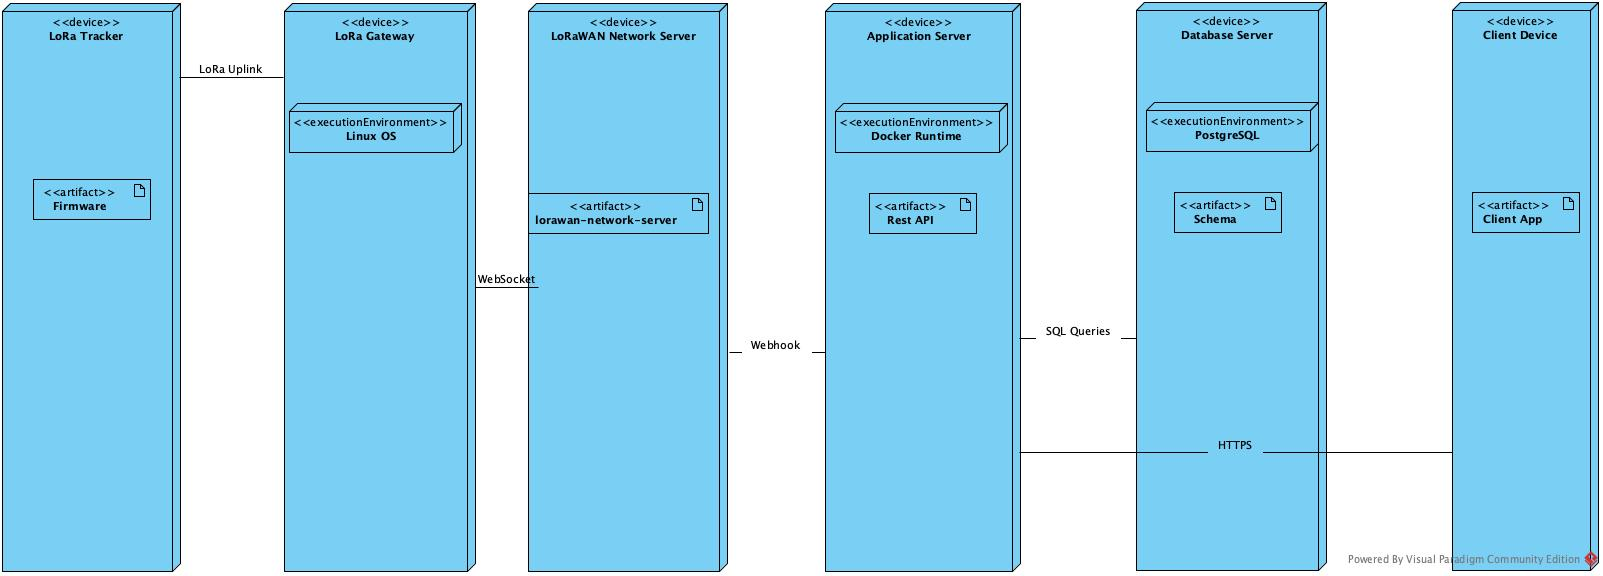
\includegraphics[width=0.7\textwidth]{png/systemOverview.jpg}
    \caption{System Diagram}
    \label{fig:SystemOverview}
\end{figure}

\subsection{Next Week's Plan}
Ryan will research open-source tracker designs; Roy will research scalability; Cory will research AWS-free workflows. We will continue debugging the LoRaWAN board.


%=======================================================
\section{Week Report 1 (09/05/2025)}
\label{sec:report1}

\subsection{Progress Made}
Ryan and Cory explored project ideas, consulted classmates and professors, and planned a decision timeline.

\subsection{Next Week's Plan}
Ryan will request continuation of his summer research project on LoRaWAN-based GPS tracking.

\subsection{Backup Plan}
If needed, the team may pivot to a “magic mirror” dashboard project driven by a Raspberry Pi.


\chapter{Development Notes \\
\small{\textit{- Ryan Davis, Cory Vitanza, and Roy Tas}}}
\index{Development Notes} 
\index{Chapter!Development Notes}
\label{Chapter::DevelopmentNotes}

\section{Wio Tracker 1110 configs}
\begin{itemize}
    \item Boards manager URL for ArduinoIDE: \url{https://files.seeedstudio.com/arduino/package_seeeduino_boards_index.json}
    \item Boards file: Seeed nRF52 Boards
    \item Seeed Wio Tracker 1110
\end{itemize}

\section{Connecting to TTN}
\begin{itemize}
    \item \url{https://wiki.seeedstudio.com/connect_wio_tracker_to_TTN/}
    \item JoinEUI=AppEUI
    \item sensecraft app for enrollment.
\end{itemize}

% ---------- References ----------
\nocite{*}
\bibliographystyle{IEEEtran}
\cleardoublepage
\phantomsection
\addcontentsline{toc}{chapter}{References}
\bibliography{bibfile}

% ---------- Index ----------
\printindex

\end{document}

